% Version: v21 -- Figure 5 integration pass
% Changes since v20: replaced the external-image placeholder for Figure 5
% (images/fig_perspectives.png, previously unrenderable/unverifiable without the asset)
% with a native TikZ diagram of the four BCHAIN-ACCESS perspectives and their intersection
% design obligations, resolving Reviewer 3's minor comment to verify Figure 5 renders
% correctly, since the figure is now generated directly by the LaTeX source with no
% external dependency.
%
% Version: v20 -- Reviewer 3 (Senior Associate Editor) revision pass
% Changes: softened non-systematic-survey equity claim (X-B); added self-constructed-rubric
% caveat to Table VII comparison (VI-E); added substantive methodological response to the
% zero-variance heuristic result and aligned it with L6 (IX-D, X-E); de-emphasized the
% feasibility-evidence contribution's evidentiary weight (I-A); added reading-guide sentence
% for cross-reference density (I); made the expert-vs-PwD caveat more prominent in the
% abstract; added explicit companion-study timeline for the PwD protocol (X-F); added an
% explicit "Scope and gating" paragraph acknowledging the editor's PwD-pilot-gating and
% paper-splitting options (X-C); fixed a pre-existing bibtex-breaking stray "@" in three
% ref.bib comments. See accompanying revision summary for the full comment-by-comment audit.
\documentclass[journal,onecolumn]{IEEEtran}
\IEEEoverridecommandlockouts
% columnsep removed for onecolumn journal format
\usepackage{array}
\usepackage{multirow}
% \usepackage{titlesec} % Removed for journal format
\usepackage{graphicx}
\usepackage{textcomp}
\usepackage{xcolor}
\usepackage{hyperref}
\usepackage{tabularx,booktabs}
\usepackage{adjustbox}
% emergencystretch set by IEEEtran
\usepackage[english]{babel}
\usepackage[font=footnotesize]{caption}
% intextsep set by IEEEtran
% titlespacing removed for IEEEtran journal format

\usepackage{cite}
\usepackage{float}
\usepackage{amsmath,amssymb,amsfonts}
\usepackage{algorithm}
\usepackage{algpseudocode}
\usepackage{tikz}
\usetikzlibrary{shapes.geometric, arrows.meta, positioning, chains}
\def\BibTeX{{\rm B\kern-.05em{\sc i\kern-.025em b}\kern-.08em
    T\kern-.1667em\lower.7ex\hbox{E}\kern-.125emX}}

\begin{document}

\title{Toward Empowering Accessibility: BCHAIN-ACCESS, an Accessibility-by-Design Framework Integrating Blockchain and HCI for Healthcare Interfaces}

\author{\IEEEauthorblockN{Nadeem Yaqub}
\IEEEauthorblockA{\textit{College of Computer Science and Technology}\\
\textit{Beijing University of Technology}\\
Beijing, China\\
nadeem.yb@gmail.com}
\and
\IEEEauthorblockN{Muhammad Sami Ullah}
\IEEEauthorblockA{\textit{Department of Computer Science}\\
\textit{Gujrat Institute of Management Sciences (GIMS), Arid University}\\
Pakistan\\
maliksami961@gmail.com}
\and
\IEEEauthorblockN{Imtiaz Hussain}
\IEEEauthorblockA{\textit{Department of Computer Science}\\
\textit{University of Management \& Technology, Sialkot Campus}\\
Pakistan\\
khan.imtiaz.ly@gmail.com}
\and
\IEEEauthorblockN{Sama Aleshaiker}
\IEEEauthorblockA{\textit{School of Computing and Engineering}\\
\textit{University of West London}\\
United Kingdom\\
sama.aleshaiker@uwl.ac.uk}
}


\maketitle

% ============================================================
% ABSTRACT
% ============================================================
\begin{abstract}
Blockchain-based healthcare systems offer secure, transparent data management, yet their adoption is constrained by usability and accessibility barriers, particularly for people with disabilities (PwDs). Despite growing interest in blockchain and Human-Computer Interaction (HCI) in healthcare, few, if any, established frameworks systematically address UI/UX design for PwDs in this context. We investigate what accessibility barriers established standards and literature predict for PwDs in blockchain healthcare interfaces, how HCI principles can address them, and what framework can guide the design of secure, regulation-compliant, accessibility-driven systems. Through a targeted narrative survey and a document-based heuristic evaluation of three blockchain healthcare applications against Nielsen's heuristics and WCAG~2.1, we identify twelve recurring barriers across four dimensions: authentication complexity, interface transparency, feedback adequacy, and assistive-technology compatibility. We propose \textbf{BCHAIN-ACCESS}, an accessibility-by-design HCI framework derived from WCAG~2.1, Nielsen's heuristics, and the accessibility literature, that integrates blockchain architecture, HCI principles, and regulatory compliance into a unified, disability-inclusive model. To demonstrate technical feasibility, a two-component reference implementation was developed: a UI-layer prototype implementing all four HCI principles, assessed by ten independent domain experts, and a blockchain backend (\texttt{HealthAccessControl.sol}, Solidity~0.8.19) executed on a local development node. \textbf{This evaluation is expert-layer only: the ten evaluators were non-disabled domain experts, not people with disabilities, and the prototype was purpose-built to the same standards against which it was scored.} The resulting expert scores are correspondingly high (for reference, mean SUS 87.5) but should be read as evidence of standards-conformant construction, not of confirmed real-world accessibility. All five expert-layer validation criteria were met at the interface level; empirical validation with PwD participants is identified as the essential next step, for which a pre-specified protocol is provided.
\end{abstract}

\begin{IEEEkeywords}
blockchain, healthcare, HCI, Accessibility, People with Disabilities, WCAG 2.1, Usability, GDPR Compliance
\end{IEEEkeywords}

% ============================================================
% SECTION I: INTRODUCTION
% ============================================================
% titlespacing removed for IEEEtran journal format
\section{Introduction}

Blockchain technology has emerged as a transformative infrastructure for healthcare data management, offering decentralization, tamper-proof record keeping, and transparent audit trails \cite{taherdoost2023role}. However, despite its technical promise, blockchain-based healthcare applications face a fundamental adoption challenge: their interfaces are reported as difficult to use, even for technically proficient users \cite{tharani2022ui,jang2020user}. For people with disabilities (PwDs), a population with heightened dependency on accessible digital health services, established accessibility standards and prior HCI research indicate that this usability gap is likely to represent a critical barrier to equitable healthcare access.

Human-Computer Interaction (HCI) research has long established that accessible, user-centered design is not optional but foundational to any technology intended for broad public use \cite{alfayez2024user}. Yet the intersection of blockchain, HCI, and healthcare accessibility remains severely underexplored. A review of existing literature indicates that blockchain healthcare studies have predominantly addressed technical concerns, consensus mechanisms, scalability, and data integrity, while UI/UX considerations have typically been treated as secondary \cite{tharani2022ui}. More critically, accessibility requirements for PwDs are rarely addressed in current blockchain healthcare design discussions \cite{khalid2023blockchain}.

We address this gap through three research questions. \textbf{RQ1} asks what usability and accessibility barriers in blockchain-based healthcare interfaces are identified by established accessibility standards and HCI literature, and which of these are predicted to disproportionately affect people with disabilities. \textbf{RQ2} asks how HCI principles can be systematically integrated into the design of blockchain-based healthcare applications to address these predicted barriers. \textbf{RQ3} asks what conceptual framework can guide the development of secure, regulation-compliant, and accessibility-driven blockchain-based healthcare systems.

To answer these questions, we conduct a targeted literature survey of Blockchain-HCI healthcare studies published between 2018 and 2025, complemented by a heuristic evaluation of representative Blockchain healthcare interface designs using Nielsen's ten usability heuristics \cite{nielsen1994usability} and the Web Content Accessibility Guidelines (WCAG 2.1) \cite{wcag21}. Based on our findings, we propose BCHAIN-ACCESS (Blockchain-based Healthcare \textbf{Access}ibility, \textbf{C}ompliance, and \textbf{C}are for \textbf{E}quitable \textbf{S}ecure \textbf{S}ystems), an accessibility-by-design HCI framework for Blockchain healthcare interfaces. Its design guidelines are derived first from WCAG~2.1, Nielsen's heuristics, and the accessibility literature, with supporting design considerations for Blockchain architecture and regulatory compliance that require separate engineering validation. People with disabilities are the framework's primary intended beneficiaries, and empirical validation with PwD users is defined as the next research phase.

\subsection{Contributions}
This work makes one primary contribution, supported by three further contributions. These are not of equal evidentiary weight: the primary framework and the two foundational/principle contributions rest on standards-based analysis, while the feasibility-evidence contribution rests on expert-layer testing only and should be read as the weakest, most provisional of the four, since it does not yet include the population the framework is designed to serve. A single-point summary of exactly what has, and has not, been evaluated is given in Table~\ref{tab:validation-summary} (Section~\ref{sec:feasibility}).
The \textbf{primary contribution} is the BCHAIN-ACCESS framework itself: an accessibility-driven HCI design model, incorporating disability-inclusive design principles, that integrates four interconnected perspectives (Healthcare, blockchain, Governance, and HCI) with measurable, standards-derived compliance criteria for the interface layer. Three further contributions establish, motivate, and demonstrate it. The first is a \textbf{foundational barrier synthesis}: a structured, survey-informed account of the usability and accessibility barriers that WCAG~2.1, Nielsen's heuristics, and prior HCI literature predict for PwDs in blockchain healthcare interfaces, organised across four dimensions (authentication complexity, interface transparency, feedback adequacy, and assistive-technology compatibility) and accompanied by a document-based mapping of existing interface patterns that identifies systematic design failures. The second is a set of \textbf{four HCI design principles} (AAD, PTD, CID, UAC) derived from this taxonomy, each mapped to specific barriers and standards, which operationalise the framework at the interface layer. The third is \textbf{expert-layer feasibility evidence}, the weakest and most provisional of the four: a two-component reference implementation comprising a WCAG~2.1 Level~AA compliant UI-layer prototype assessed by ten independent expert evaluators (Figure~\ref{fig:expert-eval}; mean SUS 87.5, 100\% expert task success, ACS 100\%) and a working blockchain backend realising the framework's technical architecture (Section~\ref{subsec:blockchain-architecture}). The two components were evaluated separately and should not be conflated: the expert assessment covers the UI-layer prototype only, whereas the blockchain backend is demonstrated but not itself independently audited or user-tested. Table~\ref{tab:prototype-vs-full} (Section~\ref{sec:implementation}) gives the full component-by-component scope breakdown against a hypothetical production system and is the clearest reference point for what has, and has not, been evaluated. A pre-specified protocol for the essential next step of PwD user validation is also provided.

The remainder of this paper is structured as follows. Section~\ref{sec:background} provides background on blockchain, HCI, and healthcare accessibility. Section~\ref{sec:methodology} presents our methodology. Section~\ref{sec:barriers} identifies and categorizes predicted usability and accessibility barriers (RQ1). Section~\ref{sec:principles} proposes HCI integration principles (RQ2). Section~\ref{sec:framework} presents the BCHAIN-ACCESS framework (RQ3), which Section~\ref{sec:operationalization} operationalizes into measurable criteria and Section~\ref{sec:implementation} realizes as a two-component reference implementation. Section~\ref{sec:feasibility} reports the expert feasibility assessment. Section~\ref{sec:discussion} discusses findings, limitations, and presents a pre-specified methodology for future PwD validation (Section~\ref{sec:pwd-validation}). Section~\ref{sec:conclusion} concludes. Given the density of cross-referencing this scope requires (barriers B1--B12, principles AAD/PTD/CID/UAC, perspectives P1--P4, validation criteria VC1--VC5), two tables are provided as navigation aids and can be consulted independently of a linear read: Table~\ref{tab:traceability} (Section~\ref{sec:framework}) traces each barrier through to its validation criterion, and Table~\ref{tab:validation-summary} (Section~\ref{sec:feasibility}) gives a single-point summary of what is, and is not, confirmed by this paper's evidence.

\subsection{Abbreviations}
Table~\ref{tab:abbreviations} summarizes the recurring abbreviations used throughout this paper for reference.

\begin{table}[htbp]
\caption{Abbreviations Used in This Paper}
\label{tab:abbreviations}
\begin{center}
\small
\begin{adjustbox}{max width=\columnwidth}
\begin{tabular}{|l|l|}
\hline
\textbf{Abbreviation} & \textbf{Meaning} \\
\hline
PwD(s) & People/Person with Disabilities \\
\hline
HCI & Human-Computer Interaction \\
\hline
WCAG & Web Content Accessibility Guidelines \\
\hline
AAD & Abstracted Authentication Design (Principle 1) \\
\hline
PTD & Progressive Transparency Design (Principle 2) \\
\hline
CID & Confirmatory Interaction Design (Principle 3) \\
\hline
UAC & Universal Assistive Compatibility (Principle 4) \\
\hline
ACS & Accessibility Compliance Score (Eq.~\ref{eq:acs}) \\
\hline
VC1--VC5 & Validation Criteria 1--5 (Section~\ref{sec:validation-criteria}) \\
\hline
GDPR & General Data Protection Regulation \\
\hline
PBFT & Practical Byzantine Fault Tolerance \\
\hline
SUS & System Usability Scale \\
\hline
DAC & Discretionary Access Control \\
\hline
DSR & Design Science Research \\
\hline
\end{tabular}
\end{adjustbox}
\end{center}
\end{table}

% ============================================================
% SECTION II: BACKGROUND
% ============================================================
\section{Background}
\label{sec:background}

\subsection{Blockchain Technology in Healthcare}
Blockchain is a distributed, decentralized, and cryptographically secured digital ledger in which data is stored in chronologically linked blocks, each containing a cryptographic hash of the preceding block, a timestamp, and transaction data \cite{taherdoost2023role}, properties that ensure immutability, transparency, and auditability, valuable in healthcare where data integrity and authorized access are paramount \cite{ehsan2022integrating}.

Of the three deployment types relevant to healthcare, \textit{Public Blockchains} are permissionless but offer limited scalability and privacy for sensitive patient data; \textit{Private Blockchains} trade decentralization for throughput and access control; \textit{Consortium Blockchains}, governed by a predefined group of authorized participants, are a commonly adopted healthcare architecture, balancing data privacy with distributed governance \cite{yaqub2025blockchain}. Smart contracts, self-executing code deployed on the blockchain, automate consent management, data access permissions, and audit logging \cite{kim2022blockchain}; consensus mechanisms such as Practical Byzantine Fault Tolerance (PBFT), common in permissioned healthcare blockchains, determine transaction validity without central authority.

Blockchain-based healthcare systems also face scalability and regulatory constraints. Public-blockchain throughput (e.g., pre-merge Ethereum: $\approx$15~TPS) remains far below healthcare data-system demands, though post-2022 upgrades and Layer-2 solutions (state channels, rollups) are narrowing this gap \cite{wood2014ethereum,yaqub2023enhancing}. More structurally, GDPR compliance is in tension with blockchain immutability: the right to erasure guaranteed under Article~17 is fundamentally incompatible with append-only ledger architectures, requiring workarounds such as off-chain storage of personal data with on-chain hash references \cite{yaqub2023enhancing}.

\subsection{Human-Computer Interaction and Accessibility}
Human-Computer Interaction (HCI) is the interdisciplinary study of the design, evaluation, and implementation of interactive computing systems for human use \cite{alfayez2024user}. Central to HCI is the principle of user-centered design (UCD), which mandates that system design be driven by the needs, capabilities, and context of the intended users throughout the development lifecycle.

Usability, a core HCI construct, is defined by ISO 9241-11 \cite{iso9241} as the extent to which a product can be used by specified users to achieve specified goals with effectiveness, efficiency, and satisfaction in a specified context of use. Nielsen's five usability components operationalize this definition as: learnability, efficiency, memorability, error prevention, and user satisfaction \cite{tharatipyakul2021user}.

Accessibility extends usability to users with disabilities, requiring that systems be perceivable, operable, understandable, and robust, the four principles of the Web Content Accessibility Guidelines (WCAG 2.1) \cite{wcag21}. WCAG 2.1 defines three conformance levels (A, AA, AAA), with Level AA representing the internationally recognized minimum standard for public-facing digital services. We adopt WCAG 2.1 as the stable Level~AA baseline that was in force throughout the study period; the more recent WCAG 2.2 (W3C Recommendation, October 2023) is backward-compatible with 2.1 and adds criteria (e.g., focus appearance, dragging alternatives, accessible authentication) that are directly relevant to this domain. We flag this as a specific limitation rather than a routine footnote: WCAG 2.2's new Success Criterion 3.3.8 (Accessible Authentication) speaks directly to this paper's most severe predicted barrier cluster, authentication complexity (B1--B3, Section~\ref{sec:barriers}), which the AAD principle (Section~\ref{sec:principles}) is designed to address. Re-auditing the baseline systems and the prototype against WCAG 2.2, rather than 2.1, would likely sharpen rather than weaken the paper's authentication-barrier findings, and is identified as the most immediately valuable direction for future standards migration, ahead of the broader relabeling implied by ``future work.'' Key WCAG 2.1 success criteria relevant to blockchain healthcare interfaces include: sufficient color contrast (1.4.3), keyboard accessibility (2.1.1), error identification (3.3.1), and authentication alternatives (3.3.4).

For PwDs, digital healthcare interfaces present compounded barriers. Motor impairments limit interaction with complex authentication workflows. Visual impairments require screen-reader compatibility and adequate contrast ratios. Cognitive impairments demand simplified navigation, plain language, and consistent feedback. These needs are systematically unaddressed in current blockchain healthcare interface designs \cite{khalid2023blockchain}.

\subsection{HCI in Blockchain Applications}
The application of HCI principles to blockchain systems is an emerging but underdeveloped research area. Elsden et al.~\cite{elsden2018making} provided the foundational typology of blockchain applications from an HCI perspective, identifying six application types and noting that most blockchain deployments prioritize technical infrastructure over user experience. Recent work has further examined digital empowerment as a driver of improved user experience in interactive system design frameworks \cite{wang2025digital}, reinforcing the case for human-centered approaches in blockchain interface development. Frohlich et al.~\cite{frohlich2022blockchain} examined trust models in blockchain systems, distinguishing social, technological, and institutional trust and concluding that current blockchain interfaces inadequately support user trust formation. Tharani et al.~\cite{tharani2022ui} conducted a systematic review of UI/UX research in blockchain applications, finding that fewer than 15\% of reviewed blockchain studies addressed interface design, and none provided accessibility evaluation for PwDs.

In the healthcare domain specifically, Jang et al.~\cite{jang2020user} studied user experience in blockchain health record systems, identifying authentication complexity and transaction feedback as primary usability barriers. Glomann et al.~\cite{Glomann2019ImprovingTB} proposed interface improvements for blockchain wallet applications, demonstrating that simplified key management workflows significantly improved task completion rates. However, neither study addressed accessibility requirements for PwDs, nor evaluated designs against established accessibility standards. This body of work indicates that the specific intersection of blockchain, healthcare, and disability-inclusive design remains a largely unaddressed gap, the gap this paper directly targets.


% ============================================================
% SECTION III: METHODOLOGY
% ============================================================
\section{Methodology}
\label{sec:methodology}

We employ a two-phase methodology to address the three research questions: (1) a targeted literature survey to identify and categorize usability and accessibility barriers (RQ1, RQ2), and (2) a document-based accessibility audit of representative blockchain healthcare interface documentation against established usability and accessibility standards (RQ2, RQ3).

The overall research process is summarized in Figure~\ref{fig:workflow}, which traces the flow from the literature survey and heuristic audit through barrier identification, principle derivation, and framework construction, to the reference implementation and its expert feasibility assessment. The dashed final stage, empirical validation with PwD participants, is defined and pre-specified (Section~\ref{sec:pwd-validation}) but not conducted in this work.

\begin{figure}[htbp]
\centering
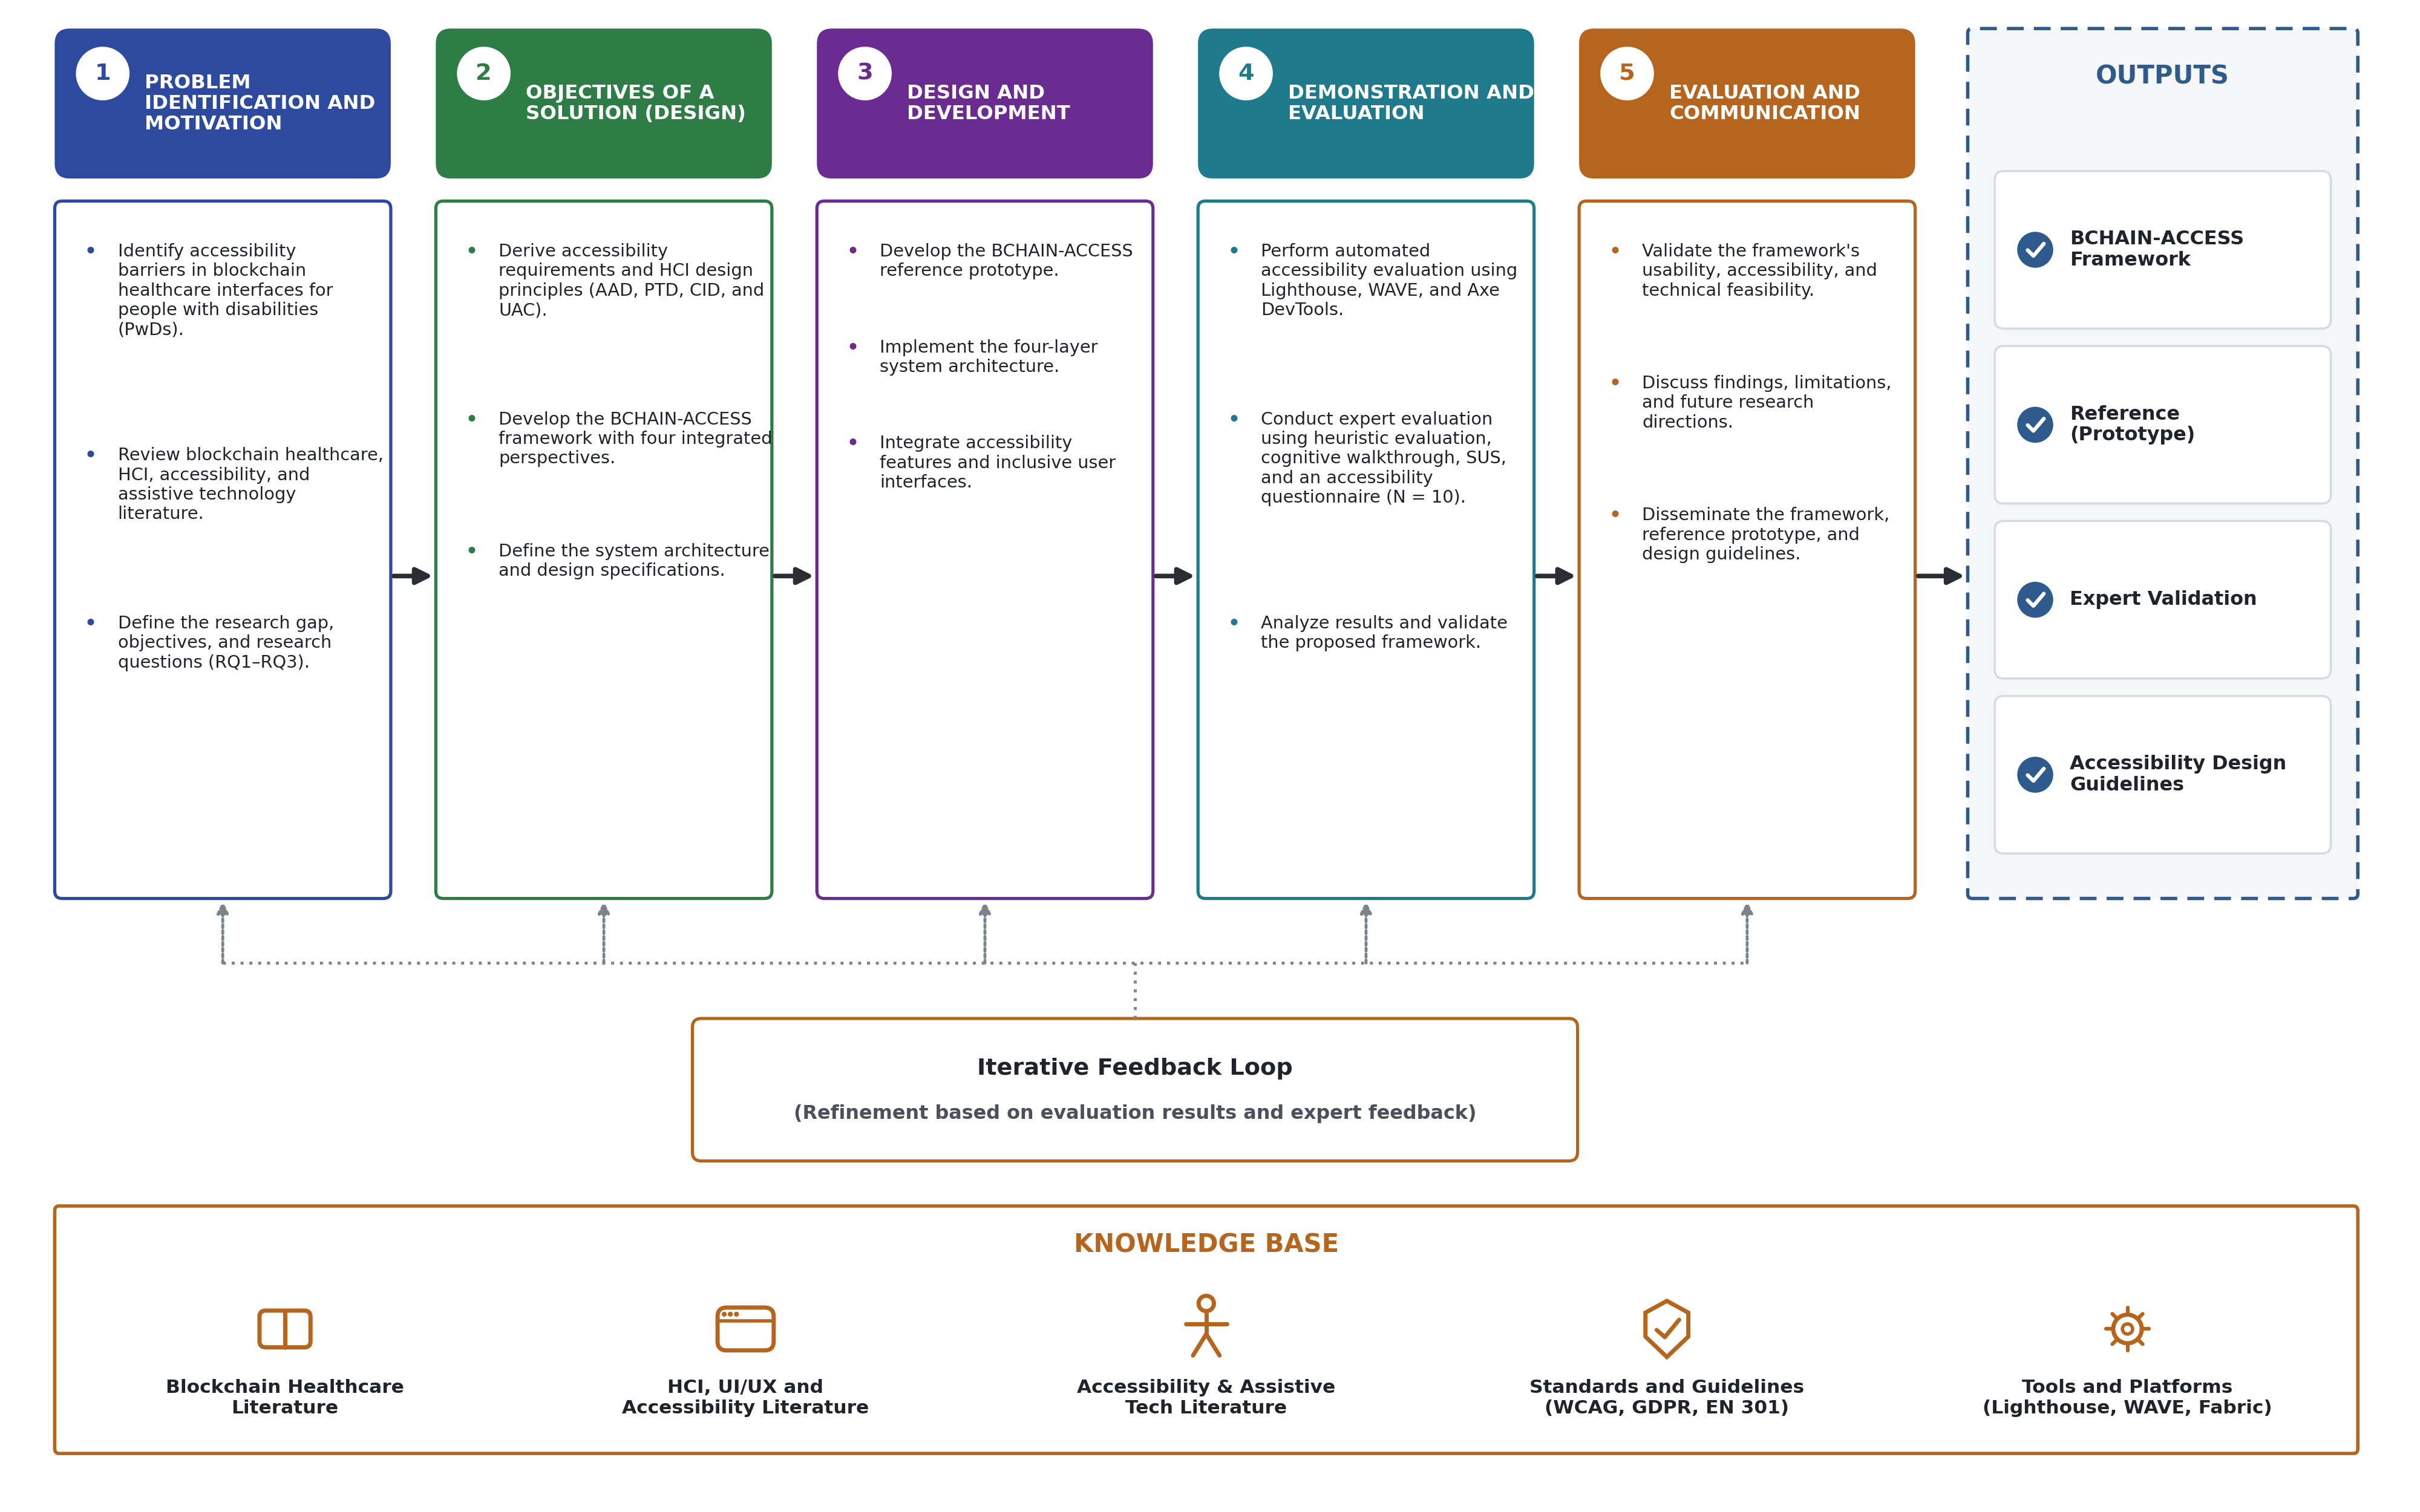
\includegraphics[width=\textwidth]{images/Figure_1.png}
\caption{Design Science Research (DSR) methodology adopted to develop and validate the BCHAIN-ACCESS framework, illustrating the five research phases, iterative refinement process, supporting knowledge base, and resulting research artifacts.}
\label{fig:workflow}
\end{figure}

\subsection{Phase 1: Targeted Literature Survey}
To motivate and contextualize the research gap addressed in this paper, we conducted a targeted, narrative survey of peer-reviewed literature on blockchain, HCI, and healthcare UI/UX published between 2018 and 2025. This survey is not a systematic literature review (SLR) in the formal methodological sense (e.g., it does not follow a pre-registered protocol, PRISMA 2020 reporting standards, or dual independent screening with inter-rater reliability reporting); it is intended to provide a representative, illustrative picture of the field sufficient to motivate and scope the research questions, not an exhaustive or fully reproducible census of the literature.

Seminal pre-2018 foundational works (e.g., MedRec \cite{medrec}, Elsden et al.~\cite{elsden2018making}) were included outside this window as primary reference systems for the heuristic evaluation. The following digital databases were searched: IEEE Xplore, ACM Digital Library, SpringerLink, and PubMed. Search strings combined terms from three clusters: a blockchain cluster (``blockchain'', ``distributed ledger'', ``smart contract'', ``decentralized''); an HCI/UI cluster (``human-computer interaction'', ``user interface'', ``usability'', ``accessibility'', ``UI/UX'', ``user experience''); and a healthcare/PwD cluster (``healthcare'', ``medical records'', ``people with disabilities'', ``assistive technology'', ``inclusive design'').

Papers were informally screened by a single reviewer (the authors) for relevance to the intersection of blockchain, HCI, and healthcare UI/UX, retaining those that: (a) addressed blockchain in a healthcare or medical context, and (b) discussed interface design, usability, or accessibility in any form. Papers addressing only blockchain infrastructure without any UI/UX component, or focused exclusively on cryptocurrency interfaces without healthcare relevance, were excluded from the retained set. Because screening was conducted by a single reviewer without a second independent rater, the retained sample should be understood as a representative, non-exhaustive snapshot rather than a fully reproducible or bias-controlled census.

Of the papers retained through this process (34 papers), only a minority, 6 papers (17.6\%), addressed any accessibility consideration for people with disabilities, an observation that is consistent with, and helped motivate, the research gap identified in RQ1. This count should be read as descriptive of our specific, non-exhaustive search rather than as a generalizable bibliometric finding about the field as a whole.

\subsection{Phase 2: Heuristic Evaluation}
\label{subsec:heuristic-eval}
We selected three systems through purposive maximum-variation sampling to identify documented interface barriers. The goal was not hands-on heuristic evaluation but a structured document-based accessibility audit of publicly available interface documentation. The objective was analytical depth rather than statistical generalization: MedRec (academic prototype), Patientory (commercial patient-engagement platform), and BurstIQ (enterprise health-data marketplace) were selected because they represent three widely cited architectural paradigms in blockchain healthcare and thereby provide maximum architectural variation. They also span the deployment spectrum and are among the few blockchain healthcare systems with sufficient public interface documentation to support barrier identification.

Because the evaluation was conducted on documentation rather than live systems, the severity ratings reported in Tables~\ref{tab:heuristic} and~\ref{tab:wcag} are proxy estimates based on documented interface patterns, not live interaction data. Barriers recurring across all three diverse contexts (e.g., universal WCAG~3.3.4 failure) are unlikely to be artifacts of any single design lineage. We acknowledge this as a purposive, non-exhaustive sample of three systems (L3), including one academic prototype (MedRec, 2016) and two commercial products evaluated through documentation from 2022--2024 and treat broader sampling as future work.

The evaluation employed two complementary frameworks. \textbf{Nielsen's Ten Usability Heuristics}~\cite{nielsen1994usability}: each application's documented interface patterns were assessed against all ten heuristics, rated on a severity scale of 0 (not a problem) to 4 (usability catastrophe). \textbf{WCAG 2.1 Level AA Criteria}: interface patterns were evaluated against the four WCAG 2.1 principles at Level AA conformance, focusing on criteria directly relevant to blockchain authentication and data interaction: color contrast (1.4.3), keyboard navigation (2.1.1), focus visibility (2.4.7), error identification (3.3.1), labels and instructions (3.3.2), and authentication alternatives (3.3.4).

Evaluation was conducted by two independent evaluators using published interface documentation, user reviews, and prior usability study reports.\footnote{Primary sources per system: MedRec, original conference paper and MIT Media Lab interface specification; Patientory, official whitepaper (v2.0, 2022) and App/Play Store reviews (2022--2024); BurstIQ, product documentation portal (accessed 2024) and usability data reported in prior work.} Inter-rater disagreements were resolved through discussion and consensus. Results are reported in Section~\ref{sec:barriers}.



Both evaluators hold postgraduate qualifications in Human-Computer Interaction and have a minimum of three years experience conducting heuristic evaluations in software usability contexts. Initial independent ratings were compared using Cohen's kappa coefficient, yielding $\kappa = 0.74$ (substantial agreement \cite{landis1977measurement}), indicating reliable and consistent application of both Nielsen's severity scale and the WCAG 2.1 conformance criteria. Of 57 rated items, 8 initial disagreements arose and all were resolved through structured discussion before final ratings were recorded. H3 (User Control) and H9 (Error Recovery) exhibited the highest initial inter-rater spread (initial ratings differing by 1 point in 2 of 3 systems each), resolved by direct reference to WCAG 2.1 criterion 2.2.1 and the architectural immutability constraint inherent to all blockchain systems. WCAG criteria 2.4.7 and 3.3.2 produced one partial-versus-pass disagreement each, resolved by consensus review of the Patientory App Store documentation.




% ============================================================
% SECTION IV: BARRIERS
% ============================================================
\section{Predicted Usability and Accessibility Barriers}
\label{sec:barriers}

This section addresses \textbf{RQ1} by presenting a structured taxonomy of barriers identified through our targeted literature survey and document-based heuristic evaluation, organized across four dimensions. These barriers are derived from WCAG 2.1 standards, Nielsen's heuristics, and prior HCI literature, all of which are specifically designed to identify conditions that disproportionately affect PwDs. No PwD participants were involved at this stage; the barriers represent predictions grounded in established accessibility science, to be confirmed through the PwD user study described in Section~\ref{sec:discussion}.

\subsection{Barrier Taxonomy}

\noindent\textbf{Dimension~1: Authentication Complexity.}\ Blockchain systems rely on cryptographic key pairs for user authentication, a mechanism fundamentally different from conventional username-password paradigms. Private key management requires users to generate, securely store, and accurately reproduce long alphanumeric strings. According to WCAG 2.1 and prior HCI research, these cognitive and motor demands are likely to disproportionately affect PwDs \cite{jang2020user}.

\textbf{B1, Key Management Burden:} Users must manage private keys independently, with no recovery mechanism in most implementations. Loss of a private key results in permanent loss of access to health records. WCAG 2.1 and cognitive accessibility literature indicate this presents a critical predicted barrier for users with cognitive impairments or memory difficulties.

\textbf{B2, Multi-Factor Authentication Complexity:} Blockchain healthcare applications frequently layer cryptographic authentication with additional verification steps. For users with motor impairments, completing multi-step authentication within session timeouts is predicted to violate WCAG 2.1 criterion 2.2.1 (Timing Adjustable).

\textbf{B3, Absence of Authentication Alternatives:} No evaluated system provided alternative authentication pathways (biometric, delegated access, or guardian-assisted authentication) compliant with WCAG 2.1 criterion 3.3.4.

\noindent\textbf{Dimension~2: Interface Transparency.}\ Blockchain's underlying processes, transaction verification, consensus, block confirmation, are invisible to users yet directly affect system responsiveness \cite{frohlich2022blockchain}.

\textbf{B4, Invisible System Status:} Transaction confirmation times ranging from seconds to minutes are not communicated to users, violating Nielsen's Heuristic~1 (Visibility of System Status).

\textbf{B5, Technical Jargon in Interface Language:} Terms such as ``gas fee'', ``wallet address'', and ``hash'' appear directly in user-facing interfaces without explanation, violating Nielsen's Heuristic~2 and WCAG 2.1 criterion 3.1.5 (Reading Level).

\textbf{B6, Opaque Data Ownership Representation:} Users cannot easily determine what data is stored on-chain versus off-chain, who has accessed their records, or what consent permissions are currently active, a transparency failure with direct GDPR compliance implications \cite{frohlich2022blockchain,yaqub2025blockchain}.

\noindent\textbf{Dimension~3: Feedback Adequacy.}\ Effective feedback is a foundational HCI requirement, particularly critical in healthcare contexts where incorrect actions may have clinical consequences \cite{tharani2022ui}.

\textbf{B7, Insufficient Error Messages:} Error messages are typically cryptographic or system-level (e.g., ``Transaction reverted: out of gas'') rather than user-actionable, violating Nielsen's Heuristic~9 and WCAG 2.1 criterion 3.3.1.

\textbf{B8, Lack of Confirmation Feedback:} Successful actions, such as granting data access to a physician, are not consistently confirmed in plain language, leaving users uncertain whether critical healthcare actions were completed.

\textbf{B9, No Undo or Reversal Mechanism:} Blockchain's immutability means erroneous transactions cannot be reversed. No evaluated system provided adequate pre-confirmation warnings, violating Nielsen's Heuristic~3 (User Control and Freedom).

\noindent\textbf{Dimension~4: Assistive Technology Compatibility.}\ Compatibility with assistive technologies, screen readers, alternative input devices, voice control, is a baseline WCAG 2.1 requirement \cite{khalid2023blockchain}.

\textbf{B10, Screen Reader Incompatibility:} Dynamic interface elements including transaction status updates are not announced by screen readers due to missing ARIA live region attributes, violating WCAG 2.1 criterion 4.1.3.

\textbf{B11, Keyboard Navigation Failures:} Complex wallet interaction workflows are not fully operable via keyboard alone, violating WCAG 2.1 criterion 2.1.1, directly excluding users with motor impairments.

\textbf{B12, Insufficient Color Contrast:} Interface elements in all three evaluated systems contained foreground-background combinations below the WCAG 2.1 Level AA minimum contrast ratio of 4.5:1.


\subsection{Barrier--Disability Mapping}

Table~\ref{tab:disability} maps each identified barrier to the primary disability category predicted by WCAG 2.1 and accessibility literature to be most severely affected. Cognitive impairments are expected to be most broadly impacted (eight barriers), followed by visual impairments (five barriers) and motor impairments (three barriers), reflecting that authentication complexity and interface transparency barriers are likely to compound across interaction modalities for users with these disabilities.

\begin{table}[htbp]
\centering
\small
\caption{Predicted Barrier--Disability Category Mapping (B1--B12), derived from WCAG 2.1 and HCI literature}
\label{tab:disability}
\begin{adjustbox}{max width=\columnwidth}
\begin{tabular}{|p{1.6cm}|*{12}{c|}}
\hline
\textbf{Disability} & \textbf{B1} & \textbf{B2} & \textbf{B3} & \textbf{B4} & \textbf{B5} & \textbf{B6} & \textbf{B7} & \textbf{B8} & \textbf{B9} & \textbf{B10} & \textbf{B11} & \textbf{B12} \\
\hline
Cognitive & $\bullet$ & $\bullet$ &  & $\bullet$ & $\bullet$ & $\bullet$ & $\bullet$ & $\bullet$ & $\bullet$ &  &  &  \\
\hline
Visual &  &  & $\bullet$ &  &  & $\bullet$ &  &  &  & $\bullet$ & $\bullet$ & $\bullet$ \\
\hline
Motor & $\bullet$ & $\bullet$ &  &  &  &  &  &  &  &  & $\bullet$ &  \\
\hline
\multicolumn{13}{l}{\footnotesize\textit{Note.} $\bullet$ = primary disability category predicted to be affected per WCAG 2.1 and accessibility literature.}\\
\multicolumn{13}{l}{\footnotesize\textit{This mapping is the authors' own categorical judgment, informed by WCAG 2.1 and the cited}}\\
\multicolumn{13}{l}{\footnotesize\textit{literature; it is not derived from empirical testing with PwD participants and is a target}}\\
\multicolumn{13}{l}{\footnotesize\textit{for confirmation in the PwD validation study (Section~\ref{sec:future-work}).}}\\
\end{tabular}
\end{adjustbox}
\end{table}

\subsection{Heuristic Evaluation Results}

Table~\ref{tab:heuristic} presents Nielsen heuristic severity ratings for the three evaluated systems (0 = not a problem; 4 = usability catastrophe). Table~\ref{tab:wcag} presents WCAG 2.1 Level AA compliance results. Figure~\ref{fig:severity} visualises the severity distribution across heuristics.

\begin{table}[htbp]
\caption{Heuristic Evaluation of Blockchain Healthcare Applications}
\label{tab:heuristic}
\begin{center}
\small
\begin{adjustbox}{max width=\columnwidth}
\begin{tabular}{|p{2.8cm}|p{0.7cm}|p{0.8cm}|p{0.7cm}|}
\hline
\textbf{Nielsen Heuristic} & \textbf{Med-Rec} & \textbf{Patient-ory} & \textbf{Burst-IQ} \\
\hline
H1: Visibility of System Status & 3 & 3 & 2 \\
\hline
H2: Match System \& Real World & 3 & 2 & 3 \\
\hline
H3: User Control \& Freedom & 4 & 3 & 4 \\
\hline
H4: Consistency \& Standards & 2 & 2 & 2 \\
\hline
H5: Error Prevention & 3 & 3 & 3 \\
\hline
H6: Recognition over Recall & 3 & 2 & 3 \\
\hline
H7: Flexibility \& Efficiency & 2 & 2 & 2 \\
\hline
H8: Aesthetic \& Minimalist Design & 2 & 1 & 2 \\
\hline
H9: Error Recovery & 4 & 3 & 4 \\
\hline
H10: Help \& Documentation & 3 & 2 & 3 \\
\hline
\textbf{Mean Severity} & \textbf{2.9} & \textbf{2.3} & \textbf{2.8} \\
\hline
\end{tabular}
\end{adjustbox}
\end{center}
\end{table}

\begin{table}[htbp]
\caption{WCAG 2.1 Level AA Compliance Evaluation}
\label{tab:wcag}
\begin{center}
\small
\begin{adjustbox}{max width=\columnwidth}
\begin{tabular}{|p{2.2cm}|p{0.6cm}|p{0.8cm}|p{0.7cm}|p{0.5cm}|}
\hline
\textbf{WCAG Criterion} & \textbf{Med-Rec} & \textbf{Patient-ory} & \textbf{Burst-IQ} & \textbf{Barr.} \\
\hline
1.4.3 Color Contrast & Fail & Fail & Fail & B12 \\
\hline
2.1.1 Keyboard Access & Fail & Partial & Fail & B11 \\
\hline
2.2.1 Timing Adjustable & Fail & Partial & Partial & B2 \\
\hline
2.4.7 Focus Visible & Partial & Pass & Partial & B11 \\
\hline
3.1.5 Reading Level & Fail & Fail & Fail & B5 \\
\hline
3.3.1 Error Identification & Fail & Partial & Fail & B7 \\
\hline
3.3.2 Labels \& Instructions & Partial & Pass & Partial & B7 \\
\hline
3.3.4 Auth Alternatives & Fail & Fail & Fail & B3 \\
\hline
4.1.3 Status Messages & Fail & Fail & Fail & B10 \\
\hline
\textbf{Pass Rate (strict)} & \textbf{0/9} & \textbf{2/9} & \textbf{0/9} & --- \\
\hline
\textbf{ACS (weighted)} & \textbf{0\%} & \textbf{38.9\%} & \textbf{11.1\%} & --- \\
\hline
\end{tabular}
\end{adjustbox}
\end{center}
{\footnotesize ACS = Accessibility Compliance Score (Eq.~\ref{eq:acs}): weighted formula giving 0.5 credit for Partial. Strict pass rate counts only full Pass.}
\end{table}

\begin{figure}[htbp]
\centering
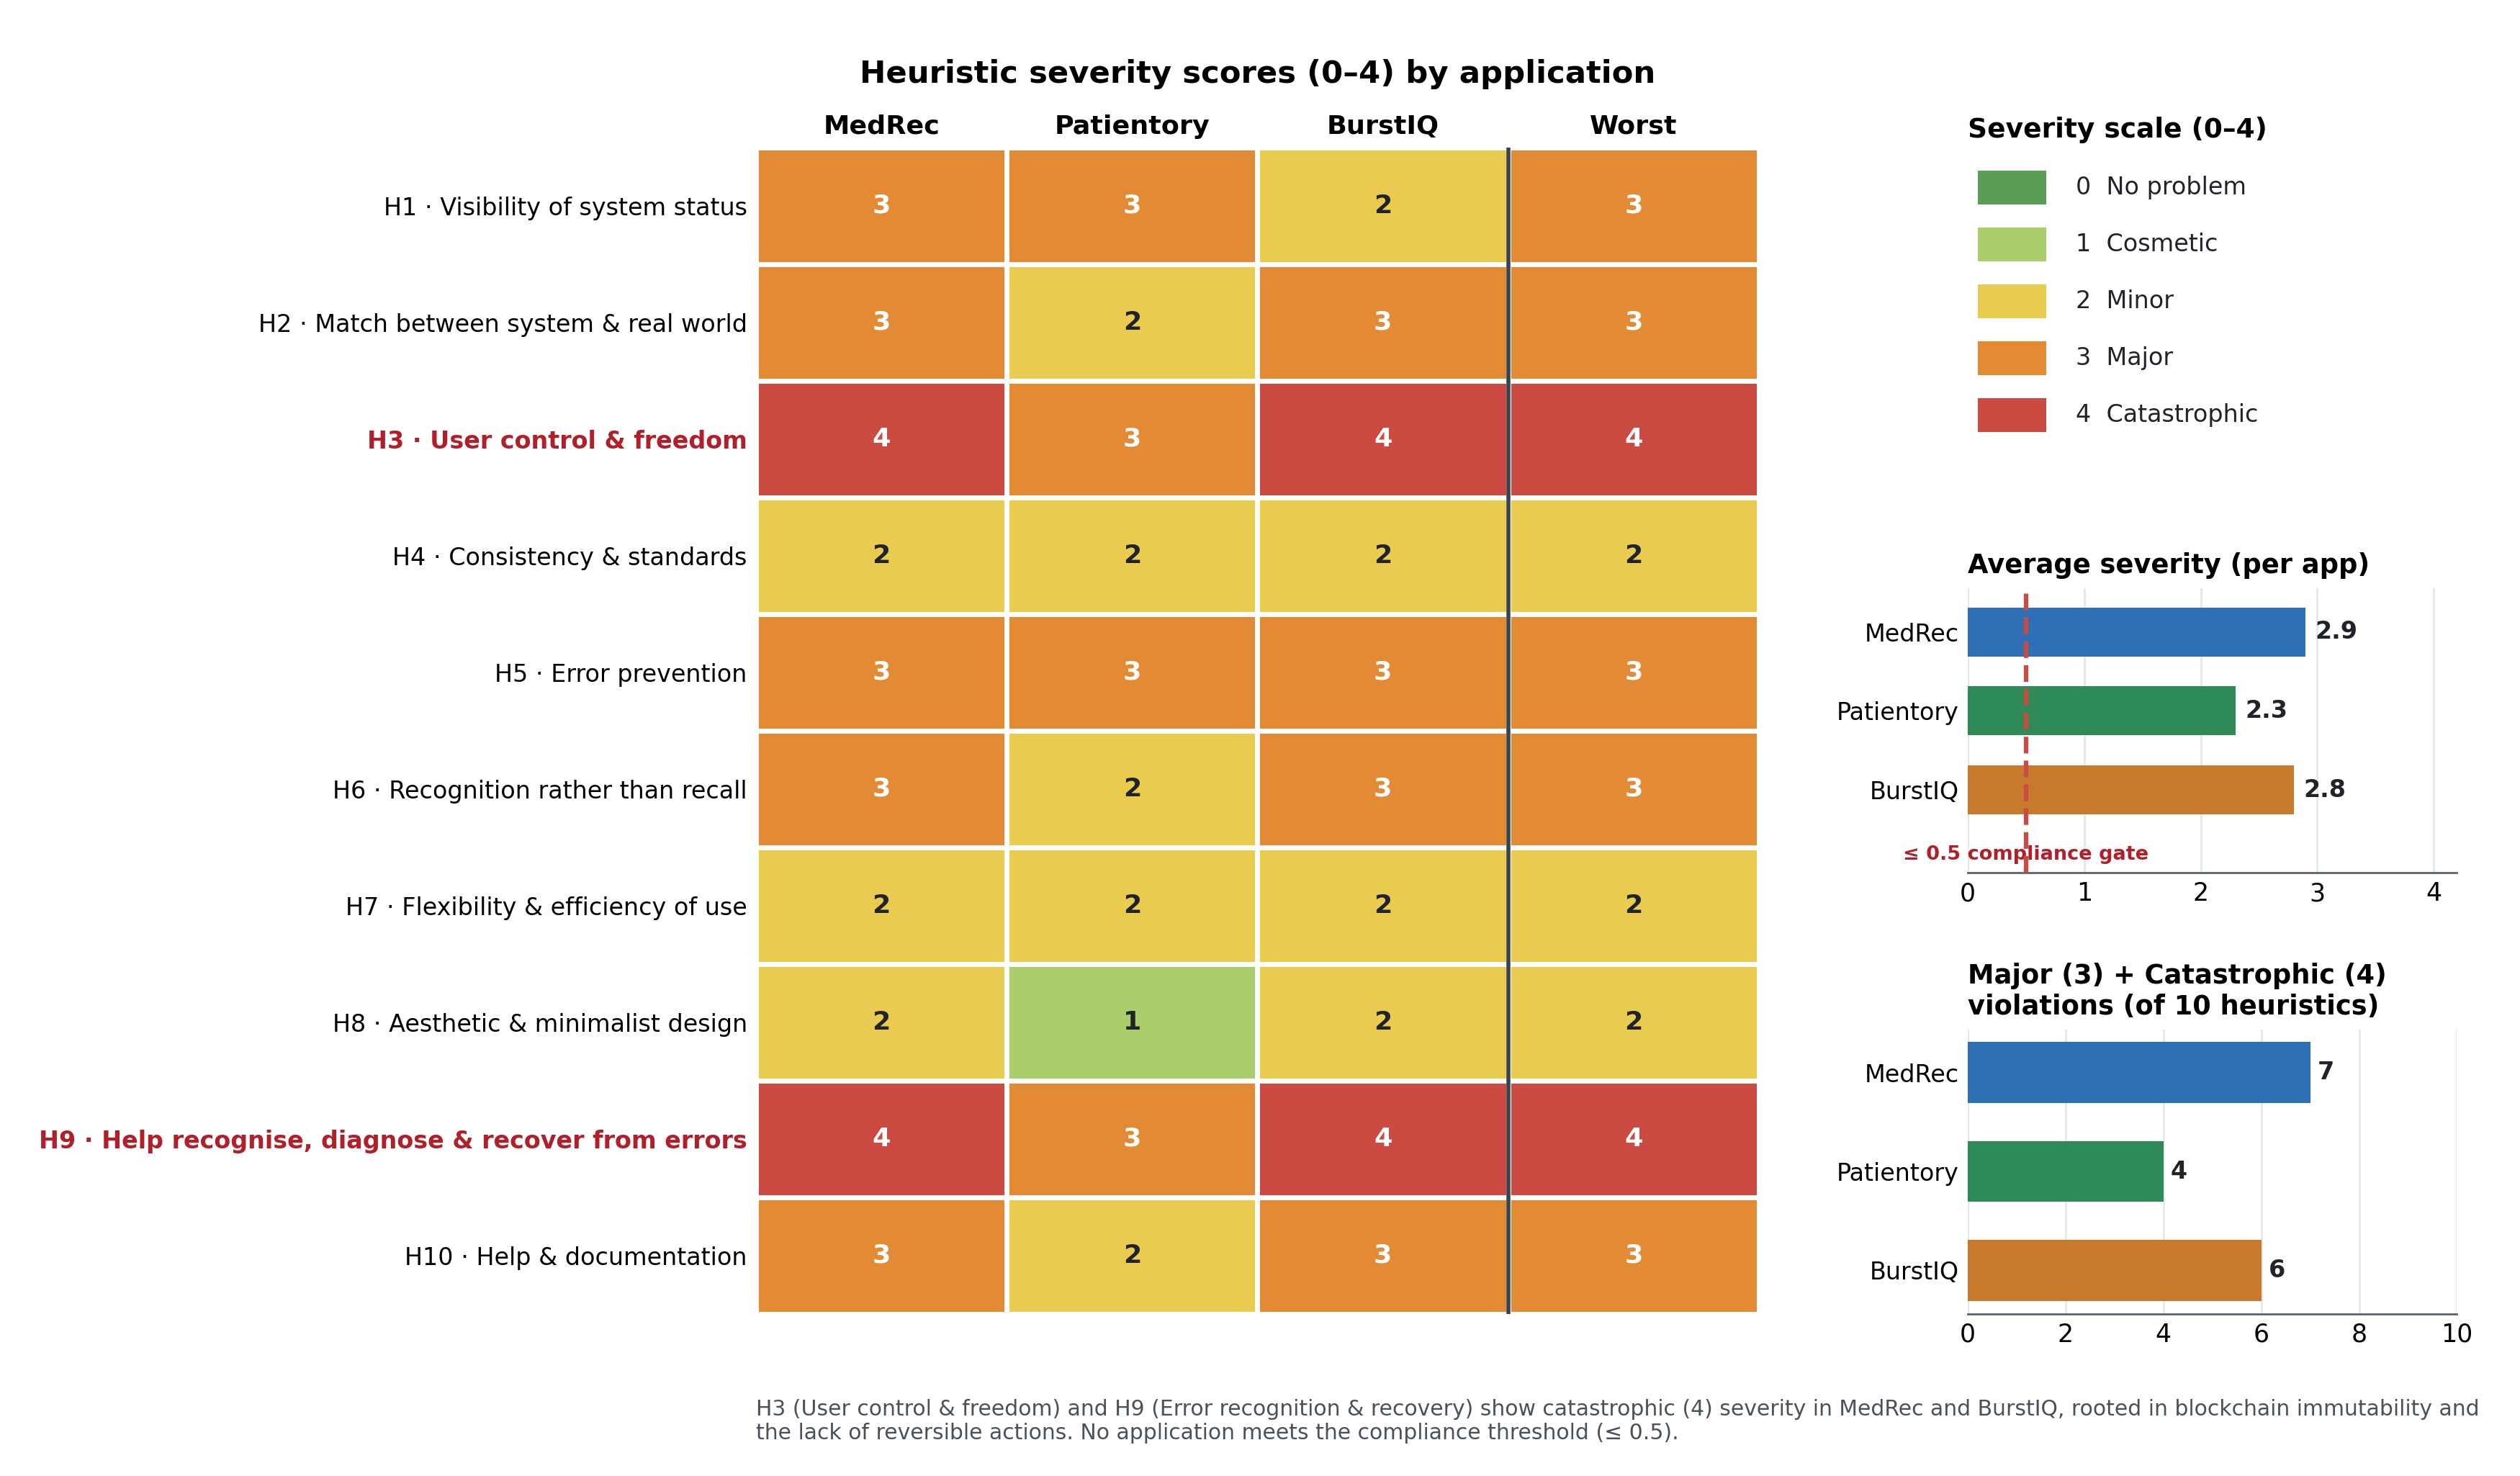
\includegraphics[width=\textwidth]{images/Figure_2.png}
\caption{Nielsen heuristic evaluation results for three representative blockchain healthcare applications, highlighting recurring usability and accessibility issues that motivate the development of the BCHAIN-ACCESS framework.}
\label{fig:severity}
\end{figure}

\subsection{Summary of Findings}
\label{sec:gap-analysis} \textbf{Finding~1, Systematic WCAG failure:} None of the three evaluated systems achieve WCAG 2.1 Level AA compliance. MedRec and BurstIQ pass zero of nine evaluated criteria (strict ACS = 0\%); Patientory achieves a strict pass rate of 22.2\% (2 of 9 criteria) and a weighted ACS of 38.9\% when partial conformance is credited. Since WCAG 2.1 criteria are specifically designed to ensure access for PwDs, these failures constitute strong standards-based evidence of predicted accessibility barriers for this population. \textbf{Finding~2, Critical severity in immutability-related heuristics:} Heuristics H3 and H9 receive catastrophic ratings (4/4) in two of three systems, reflecting structural consequences of Blockchain's immutability that standard HCI solutions cannot directly address and that are predicted to be particularly harmful for users with cognitive or motor disabilities who may be more susceptible to irreversible errors. \textbf{Finding~3, Universal authentication barrier:} All three systems fail WCAG 2.1 criterion 3.3.4 (Authentication Alternatives), indicating that, across all three evaluated systems, cryptographic key-based authentication is a barrier indicated by the standards.


% ============================================================
% SECTION V: HCI PRINCIPLES
% ============================================================
\section{HCI Integration Principles}
\label{sec:principles}

This section addresses \textbf{RQ2} by deriving four HCI design principles from the barrier taxonomy and evaluation findings. The four principles correspond directly to the four barrier dimensions identified in Section~\ref{sec:barriers} (authentication complexity, interface transparency, feedback adequacy, and assistive-technology compatibility), so that every dimension is addressed by exactly one principle; this one-to-one decomposition is a deliberate design choice to keep the framework auditable rather than a claim that no alternative grouping is possible. Each principle directly maps to one or more predicted barriers and is grounded in WCAG 2.1 and Nielsen's heuristics. The principles are designed to be implementable at the interface layer and are intended to reduce the accessibility gap for PwDs. This derivation is deductive: the four principles are constructed by the authors from the barrier taxonomy and standards, not induced from an independent dataset, and no external panel or PwD sample has yet confirmed that the four principles are jointly sufficient to close the predicted barriers. Their sufficiency, individually and jointly, is accordingly treated as a testable hypothesis of the framework rather than an established finding, and is a primary target of the PwD validation protocol (Section~\ref{sec:future-work}).

\subsection{Principle 1: Abstracted Authentication Design (AAD)}

Cryptographic authentication must be abstracted from direct user interaction through accessible intermediary mechanisms.

\textbf{Biometric key binding:} Private keys stored in secure hardware enclaves (e.g., TPM chips) unlocked via biometric authentication eliminate key string management for users with cognitive or motor impairments, addressing B1 and B2.

\textbf{Guardian-delegated access:} A structured delegation model allowing a trusted guardian to authenticate on behalf of a PwD, with auditable on-chain consent records, addresses B3 and is consistent with GDPR Article~6 provisions for consent by authorized representatives.

\textbf{Adjustable session timeouts:} Authentication sessions must be configurable per WCAG 2.1 criterion 2.2.1, with minimum 20-hour session persistence options for users who cannot re-authenticate frequently.

\subsection{Principle 2: Progressive Transparency Design (PTD)}

Blockchain's technical complexity must be disclosed progressively, revealing only what users need at each interaction stage.

\textbf{Plain language transaction status:} System status messages must translate blockchain states into user-actionable plain language, addressing B4 and satisfying Nielsen's H1.

\textbf{Layered terminology disclosure:} Technical terms must be defined inline at first use with persistent access to a plain language glossary, satisfying WCAG 2.1 criterion 3.1.5 (Reading Level) and addressing B5.

\textbf{Visual data ownership dashboard:} A screen-reader-compatible dashboard presenting on-chain versus off-chain storage status, active consent permissions, and access logs in plain language addresses B6 and supports GDPR Article~13 transparency obligations.

\subsection{Principle 3: Confirmatory Interaction Design (CID)}

Given blockchain's immutability, every consequential user action requires a structured confirmation and pre-warning workflow.

\textbf{Two-stage confirmation for irreversible actions:} All on-chain write operations must require explicit two-stage confirmation with plain language consequence statements before execution, addressing B8 and B9 and satisfying Nielsen's H3 and H5.

\textbf{Reversibility simulation layer:} Where true reversal is architecturally impossible, interfaces should implement a time-locked confirmation countdown during which a transaction is queued but not yet submitted, providing effective user control without violating blockchain integrity. The reference implementation uses a 60-second window ($\Delta = 60$s), selected to balance coercion prevention, consensus latency padding, and usability for motor-impaired users. Enforcement details at the UI and smart-contract layers are given in Section~\ref{sec:implementation}. \emph{This value was set analytically from the design rationale above, not from pilot testing with any user population.} No timing pilot (with experts or PwD participants) was conducted prior to hard-coding $\Delta = 60$s into both the UI and the smart contract. This duration is therefore a provisional default: the framework specifies that it should be user-configurable within safe bounds, and its adequacy for specific PwD groups (e.g., switch-access users) is an explicit target of the PwD validation protocol (Section~\ref{sec:pwd-validation}). Indeed, two expert evaluators (E7, E9) independently flagged the fixed countdown as a likely barrier for slower users during the feasibility assessment (Section~\ref{subsec:expert-issues}), reinforcing the need for empirical tuning rather than treating 60s as validated.

\textbf{Actionable error messages:} All error states must present: (a) plain language description of what went wrong, (b) specific user action required to resolve, and (c) contact pathway for clinical support. This addresses B7 and satisfies Nielsen's H9 and WCAG 2.1 criterion 3.3.1.

\subsection{Principle 4: Universal Assistive Compatibility (UAC)}

All interface components must be designed and tested for compatibility with the full range of assistive technologies used by PwDs.

\textbf{ARIA live region implementation:} All dynamic content updates must be implemented as ARIA live regions with appropriate politeness settings, addressing B10 and satisfying WCAG 2.1 criterion 4.1.3.

\textbf{Full keyboard operability:} Every interaction pathway must be fully operable via keyboard alone with visible focus indicators meeting WCAG 2.1 criterion 2.4.7, addressing B11.

\textbf{Contrast and visual accessibility:} All elements must meet WCAG 2.1 Level AA minimum contrast ratio of 4.5:1, with high-contrast mode support, addressing B12.

Table~\ref{tab:principles} summarizes the mapping between principles, barriers, and standards, and Figure~\ref{fig:barrier-principle-map} presents the same mapping alongside each principle's design objectives and implementation components.

\begin{table}[htbp]
\caption{HCI Principles Mapped to Barriers and Standards}
\label{tab:principles}
\begin{center}
\small
\begin{adjustbox}{max width=\columnwidth}
\begin{tabular}{|p{1.3cm}|p{1.3cm}|p{1.5cm}|p{1.5cm}|}
\hline
\textbf{Principle} & \textbf{Barriers} & \textbf{Nielsen} & \textbf{WCAG 2.1} \\
\hline
AAD & B1, B2, B3 & H5, H6 & 2.2.1, 3.3.4 \\
\hline
PTD & B4, B5, B6 & H1, H2 & 3.1.5 \\
\hline
CID & B7, B8, B9 & H3, H5, H9 & 3.3.1, 3.3.2 \\
\hline
UAC & B10, B11, B12 & H4, H7 & 2.1.1, 2.4.7, 4.1.3 \\
\hline
\end{tabular}
\end{adjustbox}
\end{center}
\end{table}

\begin{figure}[htbp]
\centering
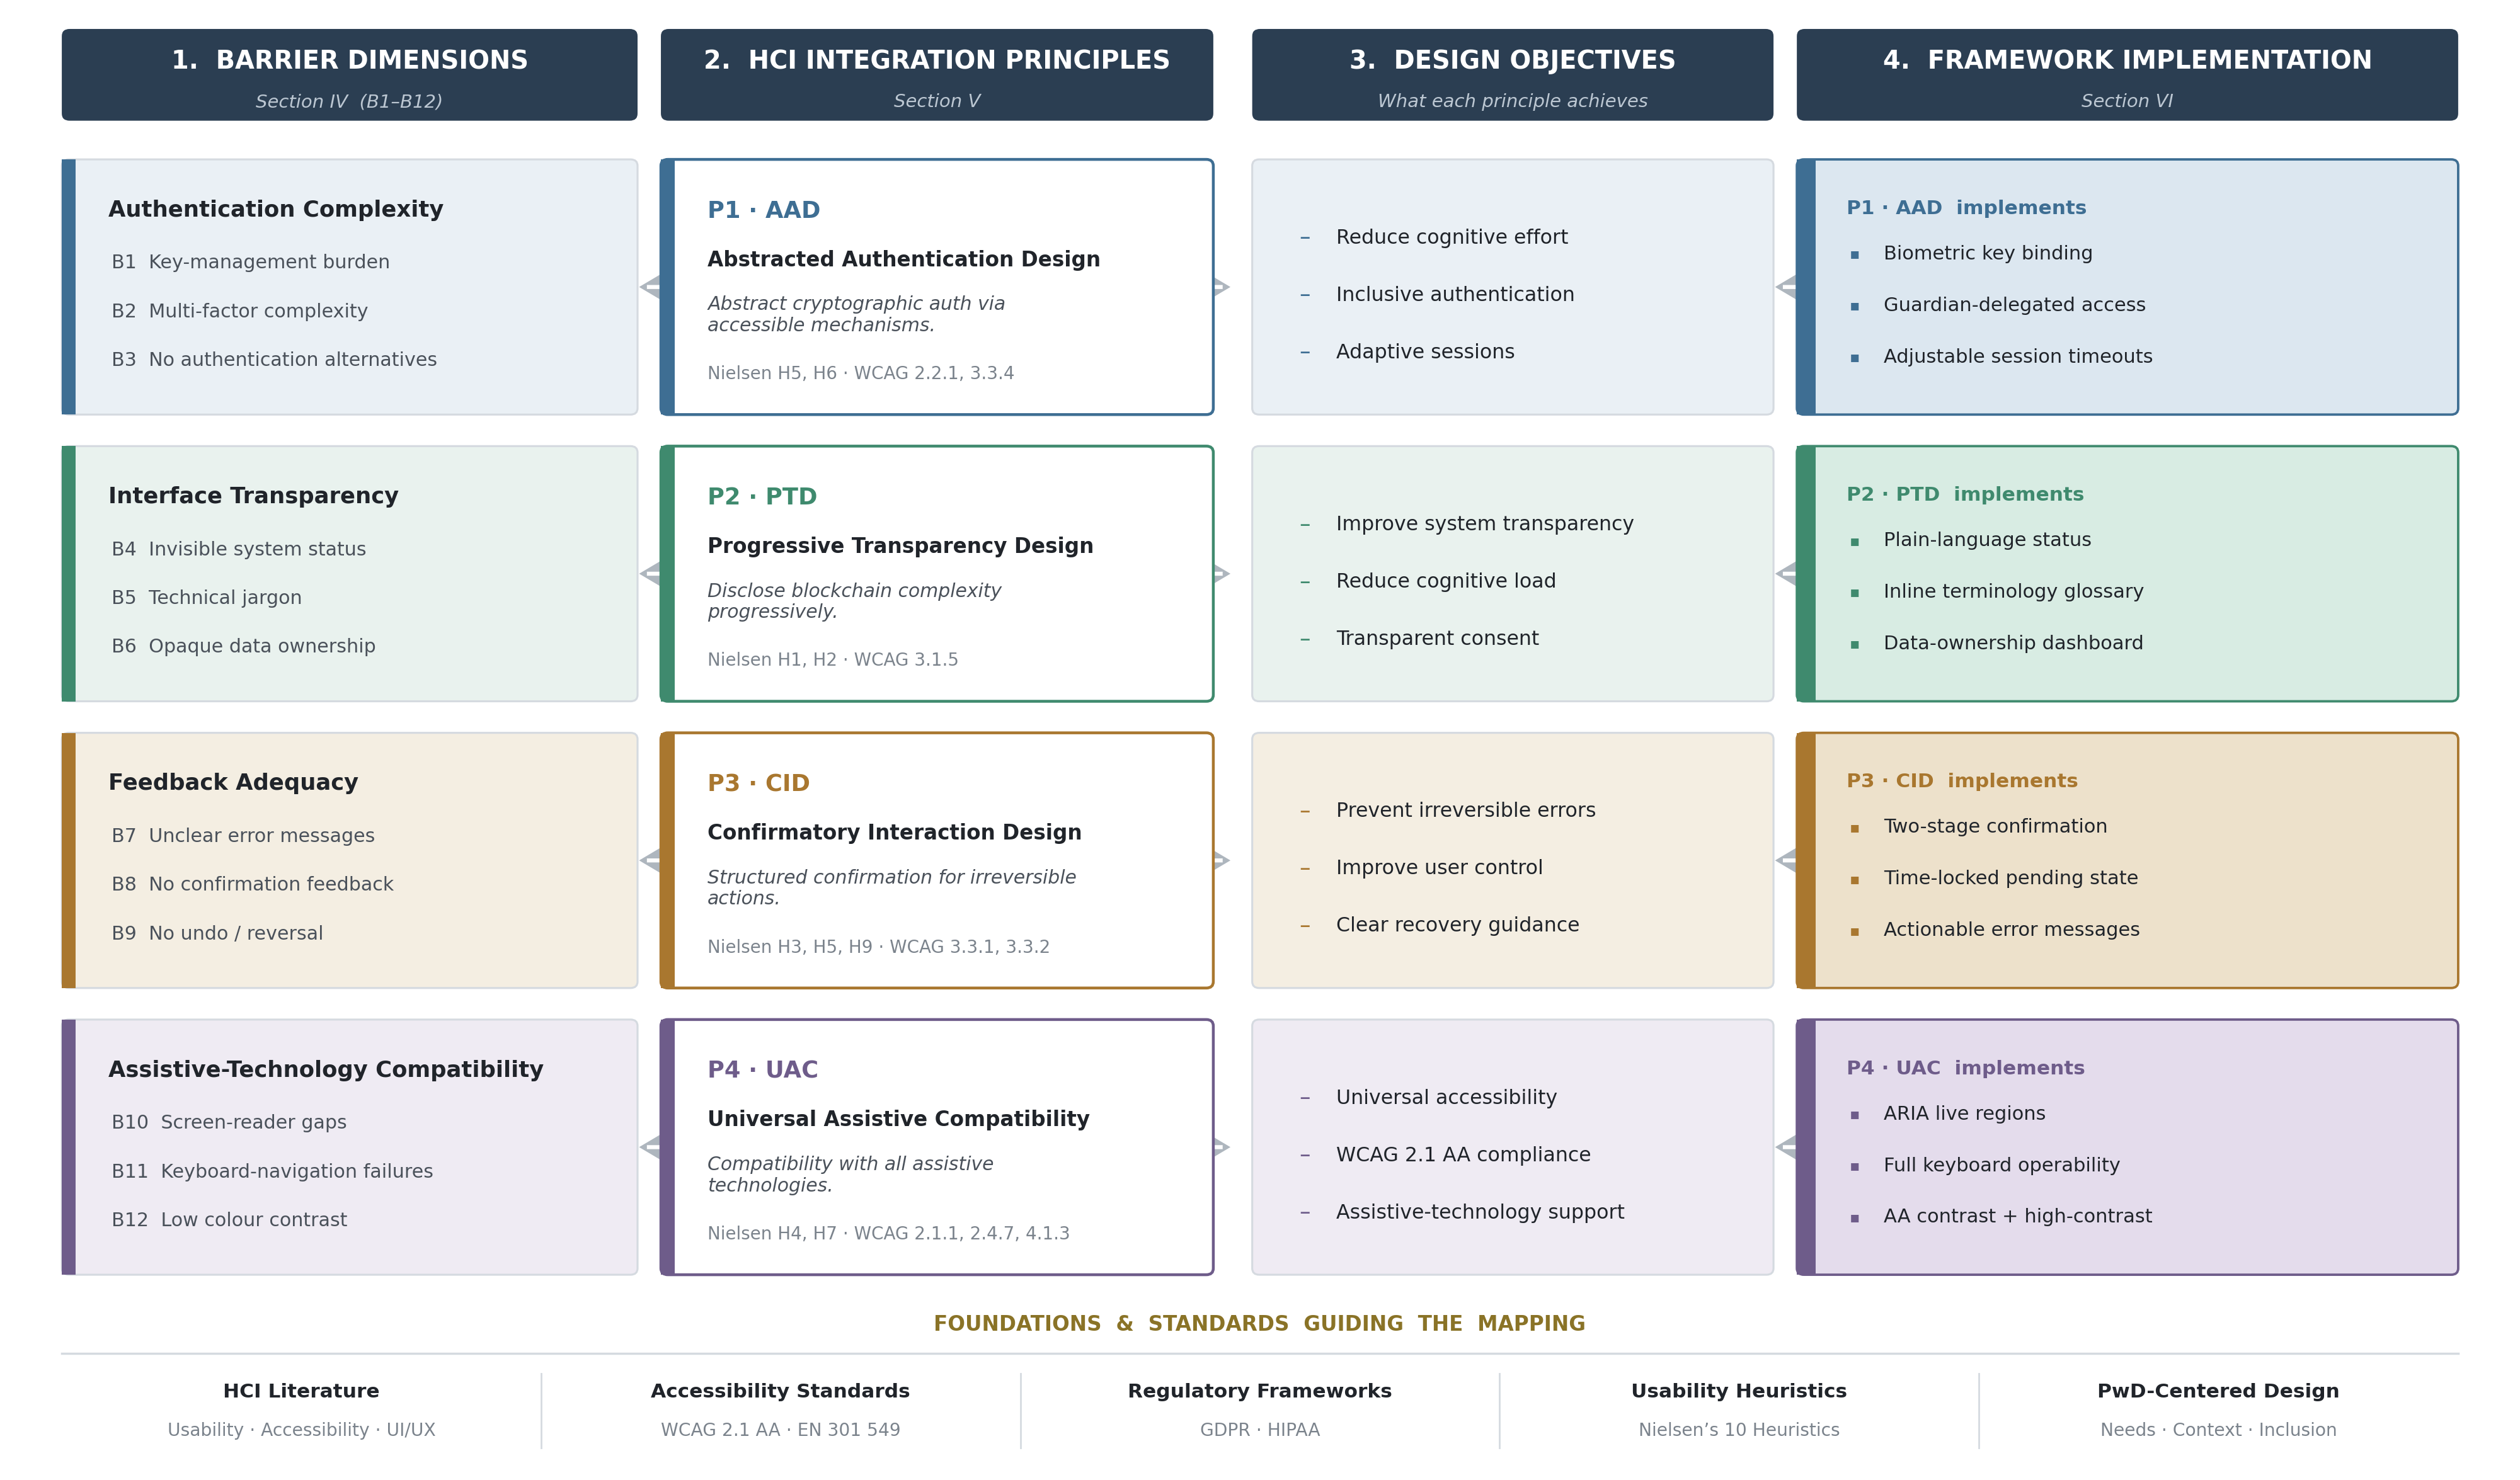
\includegraphics[width=\textwidth]{images/Figure_3.png}
\caption{Mapping of identified accessibility barriers to the BCHAIN-ACCESS design principles (AAD, PTD, CID, and UAC), corresponding design objectives, and framework implementation components.}
\label{fig:barrier-principle-map}
\end{figure}


\subsection{Illustrative Scenario}

\noindent\textit{\textbf{Hypothetical scenario (standards-based, not validated with PwD participants).}}
Consider a patient with multiple sclerosis granting her neurologist access to her MRI records. Under current MedRec design she must copy a 64-character private key (B1), authenticate within a timeout (B2), and submit an irreversible transaction with no plain-language confirmation (B8, B9). The four BCHAIN-ACCESS principles address each failure in turn: biometric unlock (AAD), a plain-language two-stage confirmation (CID), a time-locked pending state for cancellation, and an ARIA live region announcing completion (UAC). A fully worked walkthrough on the reference prototype is given in Section~\ref{subsec:case-study}.


% ============================================================
% SECTION VI: BCHAIN-ACCESS FRAMEWORK
% ============================================================
\section{The BCHAIN-ACCESS Framework}
\label{sec:framework}

This section addresses \textbf{RQ3} by presenting BCHAIN-ACCESS (Blockchain-based Healthcare \textbf{Access}ibility, \textbf{C}ompliance, and \textbf{C}are for \textbf{E}quitable \textbf{S}ecure \textbf{S}ystems). BCHAIN-ACCESS operationalizes the four HCI principles within a unified multi-perspective model, illustrated in Figure~\ref{fig:integrated}.

\begin{figure}[htbp]
\centering
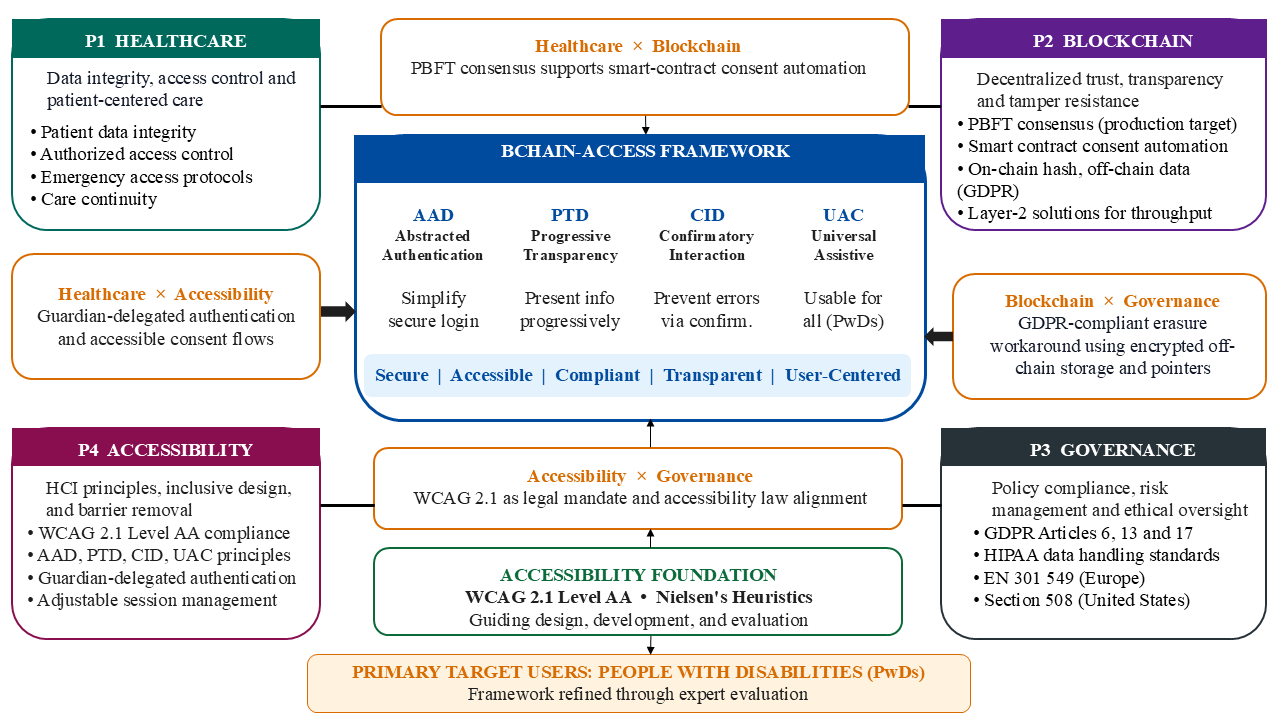
\includegraphics[width=\textwidth]{images/Figure_4.png}
\caption{Integrated BCHAIN-ACCESS framework showing the relationships among Healthcare, Blockchain, Governance, and Accessibility \& HCI perspectives, supported by accessibility-by-design principles and cross-domain interactions.}
\label{fig:integrated}
\end{figure}

\subsection{Framework Perspectives}

BCHAIN-ACCESS is organized around four interconnected perspectives, with the concrete requirements and design obligations associated with each perspective, including those arising at their intersections, shown in Figure~\ref{fig:integrated}.

\textbf{P1, Healthcare Perspective:} Defines clinical requirements including patient data integrity, authorized access control, emergency access protocols, and care continuity. At its intersection with HCI, this perspective drives accessible consent management and plain language health record presentation.

\textbf{P2, Blockchain Perspective:} Defines technical architecture including PBFT consensus for permissioned healthcare networks, smart contract design for consent automation, off-chain storage with on-chain hash verification for GDPR compliance, and Layer-2 solutions for transaction throughput. \emph{Note on the reference implementation:} PBFT consensus is a \emph{production-target} recommendation of this perspective, not a property of the reference implementation in Section~\ref{sec:implementation}, which runs on a single-node Hardhat development chain with no consensus layer (Table~\ref{tab:prototype-vs-full}). No consensus-layer prototype or roadmap artifact beyond this architectural recommendation is provided in this paper; implementing and benchmarking a PBFT (or comparable permissioned-consensus) deployment is scoped as future work alongside the public-testnet evaluation noted in Limitation~L7.

\textbf{P3, Governance and Regulatory Perspective:} Defines compliance requirements including GDPR Articles 6, 13, and 17, HIPAA data handling standards, and accessibility legislation (EN~301~549 in Europe~\cite{en301549}; Section~508 in the United States~\cite{section508}). At its intersection with HCI, this perspective mandates WCAG 2.1 Level AA compliance as a legal requirement.

\textbf{P4, HCI and Accessibility Perspective:} Incorporates the four principles defined in Section~\ref{sec:principles} (AAD, PTD, CID, UAC) as operational design requirements. At its intersection with Healthcare, this drives guardian-delegated authentication and adjustable session management for PwDs. The four perspectives are realized as the layered system architecture shown in Figure~\ref{fig:architecture}.


\begin{figure}[htbp]
\centering
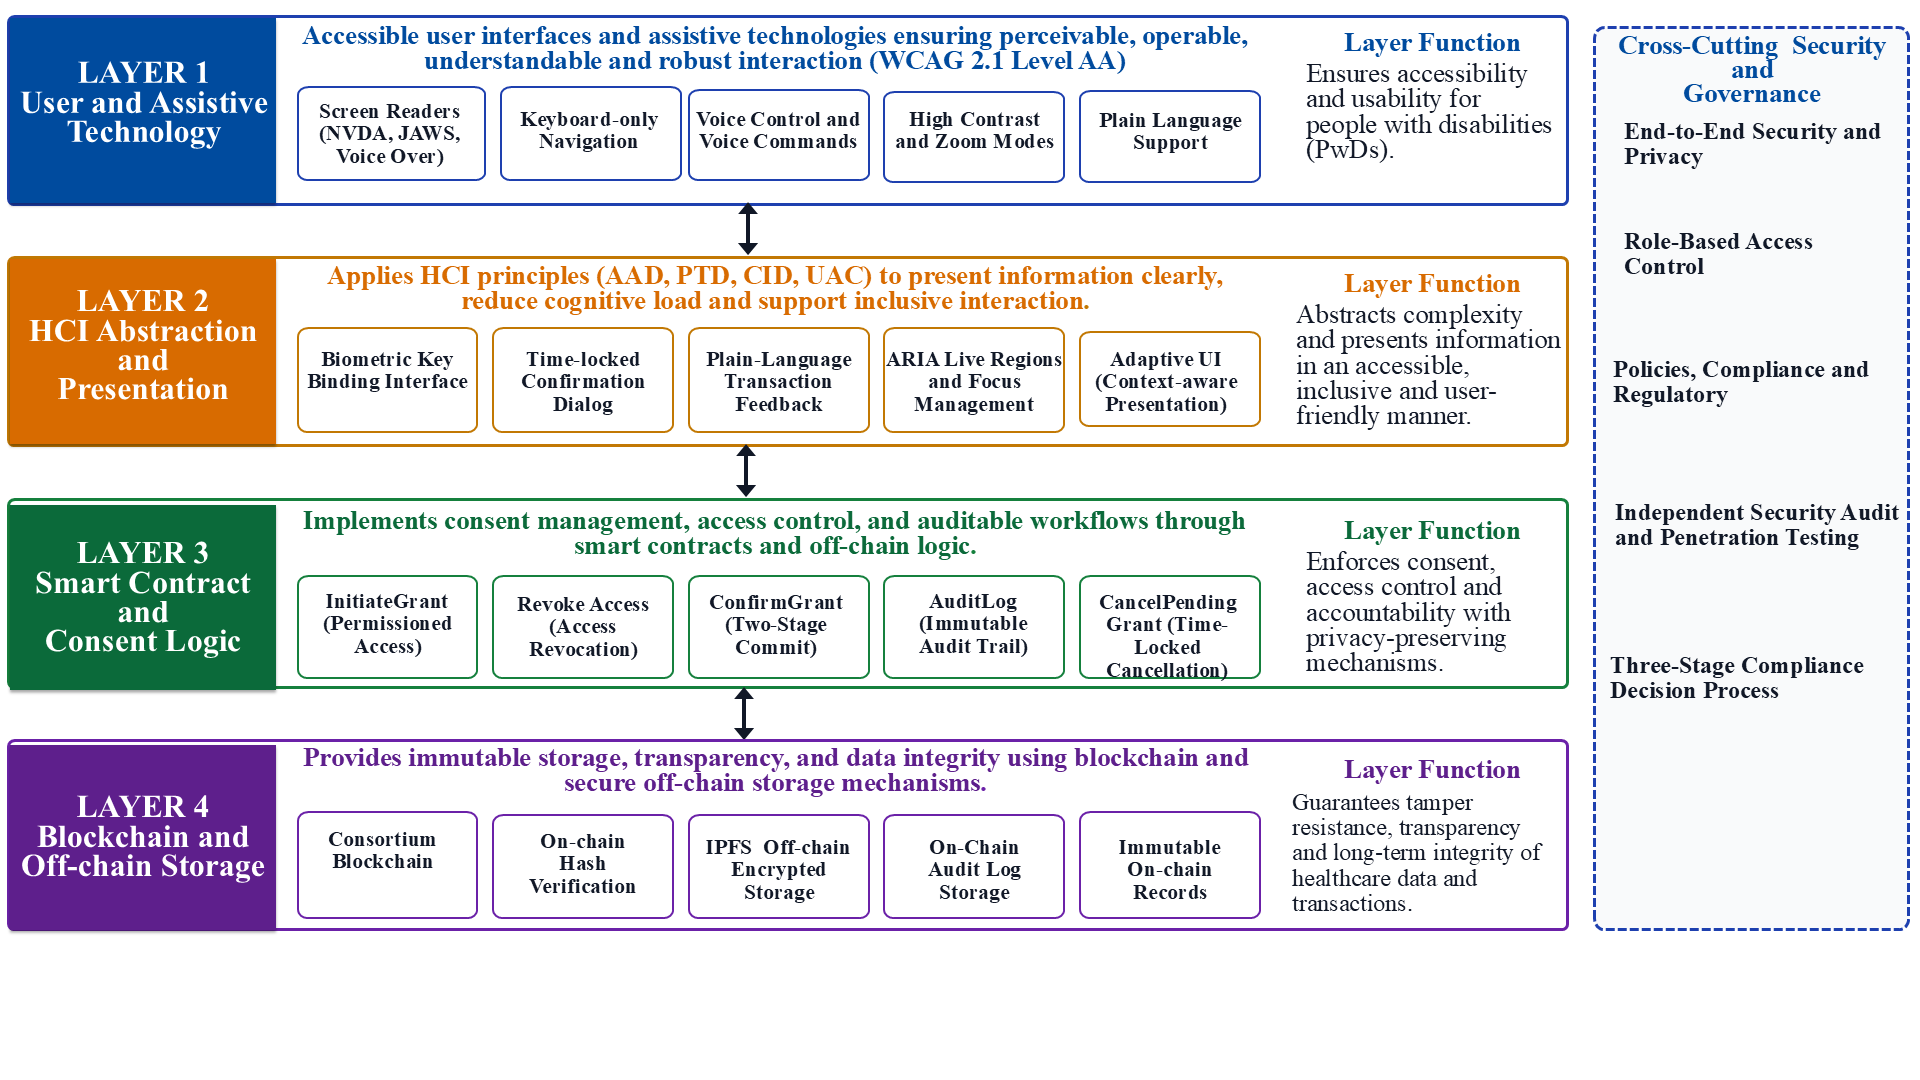
\includegraphics[width=\textwidth]{images/Figure_5.png}
\caption{Four-layer architecture of the BCHAIN-ACCESS framework comprising the User \& Assistive Technology, HCI Abstraction \& Presentation, Smart Contract \& Consent Logic, and Blockchain \& Off-chain Storage layers with cross-cutting governance and security mechanisms.}
\label{fig:architecture}
\end{figure}

\subsection{Three-Stage Decision Process}

The BCHAIN-ACCESS decision process, formalized in Algorithm~\ref{alg:bchain} (Section~\ref{sec:operationalization}), defines explicit pass/fail criteria at each stage. A ``No'' outcome at any stage halts progression and returns a remediation directive before re-entry, preventing deployment of non-compliant systems.

\textbf{Stage~1, Blockchain Security Verification:} cryptographic integrity of all health records; smart contract audit completion by an independent security reviewer; penetration testing against OWASP Blockchain Security standards; and GDPR-compatible off-chain storage architecture.

\textbf{Stage~2, Regulatory Compliance Verification:} GDPR Articles 6, 13, and 17 compliance documentation; data processing agreement (DPA) coverage for all third-party nodes; national health data regulation compliance; and accessibility legislation compliance (Section~508/EN~301~549).

\textbf{Stage~3, HCI and Accessibility Verification:} WCAG 2.1 Level AA conformance across all interface components (ACS $\geq$ 90\%); heuristic evaluation mean severity score below 0.5 across Nielsen's ten heuristics; assistive technology compatibility testing with screen readers (NVDA, JAWS, VoiceOver), keyboard-only navigation, and voice control; and usability testing with at least one PwD participant group per disability category. This final criterion is the critical empirical gate: expert evaluation and automated testing (Section~\ref{sec:feasibility}) are necessary but not sufficient, a system cannot be designated BCHAIN-ACCESS compliant without it. The complete pass/fail logic across all three stages is formalized in Algorithm~\ref{alg:bchain} (Section~\ref{sec:operationalization}).

\textbf{Compliance status of the reference implementation itself.} We flag an important scope distinction explicitly here to avoid a self-referential inconsistency. \texttt{HealthAccessControl.sol} (Section~\ref{subsec:blockchain-architecture}) has \emph{not} undergone an independent security audit, and therefore does not itself satisfy Stage~1(b) of the process just defined. No static or dynamic analysis tooling (e.g., Slither, Mythril, or fuzz-testing frameworks such as Echidna) was run against the contract in this work. Consequently, the reference implementation is presented in this paper strictly as \emph{technical realizability evidence} for the P2/P3 perspectives, i.e., a demonstration that the required functions, access-control logic, and time-locked protocol can be implemented and executed correctly, and not as a claim that the reference implementation itself has achieved, or would achieve, BCHAIN-ACCESS Stage~1 certification under its own decision process. An independent audit (even a lightweight, checklist-based static-analysis pass) of \texttt{HealthAccessControl.sol} is accordingly listed as a prerequisite for any future claim of full framework compliance, and is added explicitly to the limitations (Section~\ref{sec:discussion}, L8).

\subsection{Intersection Design Obligations}

A key contribution of BCHAIN-ACCESS is the explicit specification of design obligations arising at perspective intersections, visualized in Figure~\ref{fig:integrated}. At \textbf{Healthcare $\times$ HCI} (P1 $\times$ P4), the framework requires guardian-delegated authentication, an accessible consent UI, and plain-language health summaries. At \textbf{Blockchain $\times$ Governance} (P2 $\times$ P3), it requires off-chain storage of personal data, on-chain hash verification, and a GDPR erasure workaround. At \textbf{Governance $\times$ HCI} (P3 $\times$ P4), WCAG 2.1 Level AA becomes a legal mandate, backed by EN~301~549 compliance documentation. At \textbf{Healthcare $\times$ Blockchain} (P1 $\times$ P2), PBFT consensus supports smart-contract consent automation. Where all four perspectives converge, the framework requires the time-locked pending state and biometric key binding with an audit trail, the mechanisms that jointly implement Principles CID and AAD at the architecture level.



\subsection{End-to-End Traceability}
\label{subsec:traceability}

A central design goal of BCHAIN-ACCESS is auditability: every predicted barrier should be traceable through a principle, a standard, a concrete interface feature, and a validation criterion. Table~\ref{tab:traceability} makes this chain explicit, consolidating the mappings distributed across Sections~\ref{sec:barriers}--\ref{sec:framework} into a single matrix. This traceability is what allows the framework to be evaluated component-by-component rather than only holistically, and it defines exactly which artifact must be tested against which criterion in the PwD study.

\begin{table*}[htbp]
\centering
\small
\caption{Traceability Matrix: Barrier $\rightarrow$ Principle $\rightarrow$ Standard $\rightarrow$ Prototype Feature $\rightarrow$ Validation Criterion}
\label{tab:traceability}
\begin{adjustbox}{max width=\textwidth}
\begin{tabular}{|p{2.5cm}|p{1.0cm}|p{2.2cm}|p{3.6cm}|p{1.2cm}|p{1.6cm}|}
\hline
\textbf{Barrier} & \textbf{Principle} & \textbf{Standard (WCAG/Nielsen)} & \textbf{Prototype Feature} & \textbf{Criterion} & \textbf{Status} \\
\hline
B1 Key management; B2 MFA complexity & AAD & 2.2.1; 3.3.4; H5, H6 & Biometric-unlock button (keyboard-accessible); adjustable session & VC1, VC3 & Demonstrated \\
\hline
B3 No auth alternatives & AAD & 3.3.4 & Guardian-delegated access model; keyboard fallback & VC1 & Demonstrated \\
\hline
B4 Invisible status; B5 jargon & PTD & 3.1.5; H1, H2 & Plain-language status messages; inline glossary & VC1, VC5 & Expert layer \\
\hline
B6 Opaque data ownership & PTD & H1; GDPR Art.~13 & Visual data-ownership dashboard (screen-reader compatible) & VC1, VC5 & Expert layer \\
\hline
B7 Cryptic errors & CID & 3.3.1; H9 & Actionable plain-language error messages & VC1, VC2 & Demonstrated \\
\hline
B8 No confirmation; B9 no undo & CID & H3, H5 & Two-stage confirmation; 60-second time-locked pending state & VC2, VC3 & Expert layer \\
\hline
B10 Screen-reader incompatibility & UAC & 4.1.3 & ARIA live regions on all dynamic updates & VC1 & Demonstrated \\
\hline
B11 Keyboard failures & UAC & 2.1.1; 2.4.7 & Full keyboard operability; visible focus indicators & VC1, VC3 & Demonstrated \\
\hline
B12 Insufficient contrast & UAC & 1.4.3 & Verified $\geq$4.5:1 contrast; high-contrast mode & VC1 & Demonstrated \\
\hline
\end{tabular}
\end{adjustbox}
{\footnotesize\textit{Note.} Each row is independently testable. ``Demonstrated'' = confirmed at the prototype level by automated tooling and/or expert consensus (VC1, VC2), i.e.\ standards-conformant by construction, not validated with PwD users. ``Expert layer'' = met by expert evaluators but requiring PwD confirmation (VC3--VC5; Section~\ref{sec:pwd-validation}).}
\end{table*}

\subsection{Comparison with Existing Frameworks}


Table~\ref{tab:comparison} positions BCHAIN-ACCESS against four representative blockchain healthcare frameworks from the literature. MedRec \cite{medrec} is the foundational academic prototype; FHIRChain \cite{zhang2018fhirchain} focuses on FHIR-based interoperability; Ancile \cite{dagher2018ancile} addresses privacy-preserving EHR access control; and ACTION-EHR \cite{dubovitskaya2020action} targets cancer care data management. None of these frameworks integrates HCI design principles, accessibility evaluation, or multi-perspective design obligations. BCHAIN-ACCESS is, to our knowledge, the first framework to explicitly combine blockchain architecture, HCI principles, regulatory compliance, and disability-inclusive design into an operational model with measurable validation criteria.

\emph{Positioning of this comparison.} The seven dimensions and the resulting ratings in Table~\ref{tab:comparison} are the authors' own classification, constructed from a reading of each framework's primary publication rather than from an independent, third-party benchmarking exercise; as with any self-constructed comparison rubric, this carries some risk of framing the dimensions in ways favorable to the framework being introduced. We report it as a structured, source-grounded positioning of BCHAIN-ACCESS relative to the cited literature, not as an externally validated ranking, and we encourage readers with domain expertise to verify individual ratings against the cited primary sources listed below the table.

\begin{table*}[htbp]
\caption{Comparison of Blockchain Healthcare Frameworks}
\label{tab:comparison}
\begin{center}
\small
\begin{adjustbox}{max width=\textwidth}
\begin{tabular}{|p{2.2cm}|p{1.1cm}|p{1.1cm}|p{1.1cm}|p{1.3cm}|p{2.6cm}|}
\hline
\textbf{Dimension} & \textbf{MedRec} & \textbf{FHIRChain} & \textbf{Ancile} & \textbf{ACTION-EHR} & \textbf{BCHAIN-ACCESS} \\
\hline
HCI/UX Design & $\times$ & $\times$ & $\times$ & $\times$ & $\checkmark$ \\
\hline
Accessibility (PwD) & $\times$ & $\times$ & $\times$ & $\times$ & $\checkmark$~(design; PwD pending) \\
\hline
WCAG Compliance & $\times$ & $\times$ & $\times$ & $\times$ & $\checkmark$ \\
\hline
Regulatory Compliance & Partial & $\times$ & $\times$ & $\checkmark$ & $\checkmark$ \\
\hline
Auth.~Abstraction & $\times$ & $\times$ & $\times$ & $\times$ & $\checkmark$ \\
\hline
Usability Evaluation & $\times$ & $\times$ & $\times$ & $\times$ & $\checkmark$~(expert-layer) \\
\hline
Multi-perspective Integration & $\times$ & $\times$ & $\times$ & $\times$ & $\checkmark$ \\
\hline
\end{tabular}
\end{adjustbox}
\end{center}
{\footnotesize MedRec~\cite{medrec}: academic prototype (Azaria et al., 2016);
FHIRChain~\cite{zhang2018fhirchain}: FHIR interoperability (Zhang et al., 2018);
Ancile~\cite{dagher2018ancile}: privacy-preserving EHR (Dagher et al., 2018);
ACTION-EHR~\cite{dubovitskaya2020action}: cancer care EHR (Dubovitskaya et al., 2020).
\textbf{BCHAIN-ACCESS} is, to our knowledge, the only framework among those compared that integrates all seven dimensions with explicit disability-inclusive design; its accessibility and usability are established at the expert layer, with PwD validation pending (Section~\ref{sec:pwd-validation}).}
\end{table*}

% ============================================================
%============================================================================
% Section VII: Empirical Evaluation
% BCHAIN-ACCESS: A Blockchain Healthcare Accessibility Framework
%============================================================================

% ============================================================
% SECTION: REFERENCE IMPLEMENTATION
% ============================================================
% ============================================================
% SECTION: FRAMEWORK OPERATIONALIZATION
% ============================================================
\section{Framework Operationalization}
\label{sec:operationalization}

This section operationalizes the conceptual framework of Section~\ref{sec:framework} into measurable and implementable form: a quantitative accessibility metric, the minimum smart-contract interface, the verification algorithm, and the five validation criteria against which any candidate system, including the reference implementation of Section~\ref{sec:implementation}, is assessed.

\subsection{Accessibility Compliance Score}

To quantify WCAG 2.1 compliance unambiguously, we define the Accessibility Compliance Score (ACS) as:

\begin{equation}
\text{ACS} = \frac{N_{\text{pass}} + 0.5 \times N_{\text{partial}}}{N_{\text{total}}} \times 100\%
\label{eq:acs}
\end{equation}

\noindent where $N_{\text{pass}}$ is the number of criteria rated Pass, $N_{\text{partial}}$ the number rated Partial, and $N_{\text{total}}$ the total criteria evaluated. Applying Equation~(\ref{eq:acs}) to Table~\ref{tab:wcag}: MedRec ACS = 0\%; Patientory ACS = $(2 + 0.5\times3)/9 \times 100 = 38.9\%$; BurstIQ ACS = $(0 + 0.5\times2)/9 \times 100 = 11.1\%$. The strict pass rate (counting only full Pass, excluding Partial) is 0\%, 22.2\%, and 0\% respectively. VC1 requires ACS $\geq$ 90\% for BCHAIN-ACCESS compliance. The 90\% threshold is set deliberately below 100\% to accommodate criteria that are architecturally constrained by blockchain immutability (e.g., limited undo, reflected in the residual H9 severity) while still requiring near-complete Level~AA conformance; all three baseline systems fall substantially below this threshold.

The $0.5$ partial-credit weight is a deliberate design choice rather than an empirically fitted parameter: it reflects the common convention in conformance-auditing practice that a criterion partially met (e.g., correct on most but not all interactive elements) represents materially more accessibility than a full Fail but should not be credited as equivalent to a full Pass. We do not claim this weighting is uniquely optimal, and it has not been validated against an external, independently-derived accessibility metric. To mitigate this construct-validity concern, we report the strict (Pass-only) rate alongside the weighted ACS throughout the paper (Tables~\ref{tab:wcag} and~\ref{tab:wcag-heuristic}), so that readers who prefer a stricter, unweighted criterion can evaluate compliance without relying on the 0.5 weighting at all. Sensitivity analysis using alternative weights (e.g., 0.25 or 0.75 credit for Partial) is identified as future work for establishing the metric's robustness.


\subsection{Smart Contract Interface Specification}

The minimum smart-contract interface required by BCHAIN-ACCESS for consent management, five functions (\texttt{initiateGrant}, \texttt{confirmGrant}, \texttt{revokeAccess}, \texttt{checkAccess}, \texttt{getAuditLog}) supporting the time-locked pending state of Principle CID, is specified in full in the supplementary materials. The commit-reveal pattern underpinning \texttt{initiateGrant} and \texttt{confirmGrant} is adapted from time-lock mechanisms established in financial blockchain applications \cite{buterin2014ethereum}, here applied to healthcare consent workflows. Security note: all functions must implement role-based access control modifiers and be subject to formal verification or independent audit prior to deployment; reentrancy guards are required for all state-modifying functions. \texttt{HealthAccessControl.sol} implements the role-based modifiers and reentrancy guards described here, but, as clarified in Section~\ref{sec:framework} and Limitation~L8, has not itself undergone the independent audit this note requires.




\subsection{BCHAIN-ACCESS Verification Algorithm}

Algorithm~\ref{alg:bchain} formalises the three-stage decision process as a sequential verification procedure. Each stage is a blocking gate: failure at any stage halts progression and returns a remediation directive.

\begin{algorithm}
\caption{BCHAIN-ACCESS three-stage compliance verification}
\label{alg:bchain}
\begin{algorithmic}[1]
\Require System $S$ with architecture $A$, interface $I$, documentation $D$
\Ensure Compliance verdict $V \in \{\text{Compliant},\text{Non-compliant}\}$

\State \textbf{Stage 1 --- Blockchain security}
\If{cryptographic integrity of $A$ verified \textbf{and} smart contract audit passed \textbf{and} GDPR off-chain architecture confirmed}
    \State proceed to Stage 2
\Else
    \State $V \leftarrow$ Non-compliant; \textbf{return} architectural remediation directive
\EndIf

\State \textbf{Stage 2 --- Regulatory compliance}
\If{GDPR Arts.\ 6, 13, 17 documented \textbf{and} DPAs cover all nodes \textbf{and} EN~301~549 / Section~508 compliance confirmed}
    \State proceed to Stage 3
\Else
    \State $V \leftarrow$ Non-compliant; \textbf{return} legal remediation directive
\EndIf

\State \textbf{Stage 3 --- HCI and accessibility}
\If{$\text{ACS}(I) \geq 90\%$ \textbf{and} mean Nielsen severity $\leq 0.5$ \textbf{and} AT compatibility confirmed \textbf{and} PwD task completion $\geq 80\%$}
    \State $V \leftarrow$ Compliant; \textbf{return} BCHAIN-ACCESS certification
\Else
    \State $V \leftarrow$ Non-compliant; \textbf{return} HCI remediation directive
\EndIf
\end{algorithmic}
\end{algorithm}

\subsection{Validation Criteria}
\label{sec:validation-criteria}

BCHAIN-ACCESS provides five measurable validation criteria. Criteria VC1 and VC2 are demonstrated at the expert evaluation layer in this paper. Criteria VC3, VC4, and VC5, while met by expert evaluators in Section~\ref{sec:feasibility}, require replication with PwD participants before they can be considered confirmed for the target population. These criteria are presented as testable targets for the PwD validation study described in Section~\ref{sec:discussion}.

\textbf{VC1, Accessibility Score (ACS):} ACS (Equation~\ref{eq:acs}) $\geq$ 90\% across all evaluated WCAG 2.1 Level AA criteria. \textit{Expert-layer result: ACS = 100\% on the UI prototype} (baseline: MedRec 0\%, Patientory 38.9\%, BurstIQ 11.1\%).

\textbf{VC2, Usability Severity:} Mean Nielsen heuristic severity $\leq$ 0.5 across all ten heuristics. \textit{Expert-layer result: mean severity = 0.1 on the coarse 0--4 scale and 0.30 on a finer-grained re-rating, both within threshold} (baseline: MedRec 2.9, Patientory 2.3, BurstIQ 2.8).

\textbf{VC3, Task Success Rate:} $\geq$ 80\% task completion for core healthcare workflows in usability testing. \textit{Expert-layer result: 100\% by expert evaluators; PwD confirmation required.}

\textbf{VC4, System Usability Score (SUS):} Mean SUS score $\geq$ 68 on the standard 10-item SUS. \textit{Expert-layer result: mean SUS = 87.5 by expert evaluators; PwD confirmation required.}

\textbf{VC5, Accessibility Questionnaire:} Mean post-evaluation accessibility questionnaire rating $\geq$ 3.5/5.0. \textit{Expert-layer result: mean = 4.44/5.0 by expert evaluators; PwD confirmation required.}

\section{Reference Implementation}
\label{sec:implementation}

\subsection{Reference Implementation and Prototype Evaluation}

To demonstrate the achievability of the BCHAIN-ACCESS framework, we developed two complementary implementation components: (1) a \textbf{UI-layer prototype} used as the subject of the expert accessibility and usability evaluation, and (2) a \textbf{full blockchain backend system} implementing the technical architecture specified in Section~\ref{subsec:blockchain-architecture}. These are distinct artifacts with distinct purposes, and it is important to delineate them clearly.

\textbf{Component 1, UI-Layer Prototype (Evaluation Subject).} The UI-layer prototype is a single-page HTML/CSS/JavaScript application implementing all four HCI principles (AAD, PTD, CID, UAC) for the patient data sharing scenario described in Section~\ref{sec:principles}. It is a \textbf{self-contained presentation-layer demonstration}: all state is managed in browser memory (JavaScript variables); reloading the page resets all data. The ``fingerprint'' authentication is a keyboard-accessible button with a CSS animation simulating biometric unlock (AAD); the ``60-second countdown'' is a JavaScript \texttt{setInterval} with ARIA live region announcements (CID); ``access grants'' are managed as DOM state with plain-language confirmation dialogs (PTD); and all interactive elements are fully keyboard operable with visible focus indicators and high-contrast mode support (UAC). This component was submitted to the N=10 expert feasibility assessment reported in Section~\ref{sec:feasibility}. All color combinations were verified to meet the WCAG~2.1 Level~AA minimum contrast ratio of 4.5:1, and all interactive elements were tested for keyboard operability and screen-reader announcement. Accessibility claims (ACS = 100\%, Lighthouse 100/100) apply \textbf{solely to this HCI presentation layer}, not to any blockchain system, smart contract, or production healthcare application.

\textbf{Component 2, Full Blockchain Backend (Technical Implementation).} In parallel with the UI-layer prototype, a complete blockchain backend was implemented to demonstrate that the framework's technical architecture (P2, Blockchain Perspective; P3, Governance Perspective) is realizable. This system comprises the \texttt{HealthAccessControl.sol} Solidity smart contract executed on a local Hardhat EVM development node, and a Python Flask REST API gateway integrating via Web3.py that builds, signs, and submits transactions to the node. When the local node is unavailable, the gateway falls back to an in-memory ledger engine that preserves the same API surface for offline demonstration; all on-chain results reported in this paper were obtained from the Hardhat node. A live reference deployment of the prototype is publicly accessible at \url{https://bchain-access-frontend.onrender.com/}; permanent deployment instructions and all source code are provided in the supplementary materials. The technical details of this backend are presented in Section~\ref{subsec:blockchain-architecture}; it was not the subject of the N=10 expert evaluation, which focused on the HCI presentation layer.

\textbf{Scope of the evaluation.} The expert feasibility assessment (Section~\ref{sec:feasibility}) evaluates Component~1 (the UI-layer prototype) exclusively. Table~\ref{tab:prototype-vs-full} clarifies the boundary between the evaluated UI prototype and the full production-grade system it is designed to represent at the interface layer.

\begin{table}[htbp]
\centering
\small
\caption{Implementation Scope: UI-Layer Prototype (Evaluated) vs. Blockchain Backend (Implemented) vs. Full Production System}
\label{tab:prototype-vs-full}
\begin{adjustbox}{max width=\columnwidth}
\begin{tabular}{|p{2.8cm}|p{3.8cm}|p{3.8cm}|p{3.8cm}|}
\hline
\textbf{Component} & \textbf{UI-Layer Prototype (Evaluated, Component~1)} & \textbf{Blockchain Backend (Implemented, Component~2)} & \textbf{Full Production System (Future Work)} \\
\hline
\textbf{Blockchain Layer} & None. Client-side HTML/CSS/JS only. & \texttt{HealthAccessControl.sol} executed on a local Hardhat EVM development node via Web3.py, with an in-memory fallback ledger for offline demonstration. & Distributed ledger (e.g., Ethereum mainnet or Hyperledger Fabric) with consensus nodes and immutable transaction log. \\
\hline
\textbf{Smart Contracts} & None. No deployed code. & \texttt{HealthAccessControl.sol} (Solidity~0.8.19) compiled and deployed to local Hardhat node at \texttt{0x5FbDB...}. & Formally verified, audited Solidity contracts deployed to production EVM chain. \\
\hline
\textbf{Cryptography} & None. No hashing, signing, or encryption. & SHA-256 record hashes (salt generated and stored off-chain alongside the encrypted record, not on-chain or in cleartext transit), EVM account nonces, transaction signing via Web3.py using patient private key. & Full ECDSA secp256k1 key pairs, Merkle proofs, hardware security module (HSM) key and salt storage. \\
\hline
\textbf{Wallet Integration} & None. No Web3 or key management. & Patient wallet derived from Hardhat test account; transactions signed and submitted via \texttt{send\_contract\_tx()} in Flask backend. & User-controlled wallets (MetaMask, WalletConnect), key derivation, secure enclave storage. \\
\hline
\textbf{Data Persistence} & Browser memory only. Reload resets all state. & In-memory Python dictionaries synchronized to on-chain state via \texttt{sync\_records\_to\_\allowbreak smart\_contract()} on server startup. & On-chain transaction log + PostgreSQL off-chain metadata + IPFS encrypted storage. \\
\hline
\textbf{Authentication} & CSS-animated button (simulated fingerprint). & Simulated fingerprint in UI layer; on-chain identity enforced by wallet address and \texttt{onlyPatient()} modifier. & WebAuthn/FIDO2 biometric + cryptographic key pair, multi-factor authentication. \\
\hline
\textbf{API Gateway} & Not applicable. & Python Flask REST API (19 endpoints) connecting frontend to Hardhat EVM via Web3.py. & FastAPI/Express with PostgreSQL, Redis session caching, rate limiting, TLS 1.3. \\
\hline
\textbf{Transaction Finality} & DOM visibility toggle (no actual transaction). & EVM transactions executed and confirmed on the local Hardhat development node; gas consumption recorded from that node (reported in the supplementary materials). & Blockchain transaction with mainnet gas fees, confirmation blocks, and irreversibility. \\
\hline
\textbf{Accessibility Claim} & WCAG 2.1 AA on the UI layer only (evaluated). & Not separately evaluated; UI layer is shared with Component~1. & WCAG 2.1 AA on UI + accessible key management + screen-reader-compatible wallet flows. \\
\hline
\multicolumn{4}{|p{11.4cm}|}{\footnotesize\textit{Note.} The UI-layer prototype (Component~1) was the subject of the N=10 expert feasibility assessment. The blockchain backend (Component~2) illustrates the technical realizability of the P2 and P3 framework perspectives on a local development node. Production-grade deployment remains future work.} \\
\hline
\end{tabular}
\end{adjustbox}
\end{table}

The prototype was subsequently subjected to a full $N=10$ expert feasibility assessment comprising automated accessibility auditing, expert heuristic evaluation, a cognitive walkthrough, the System Usability Scale, and a post-evaluation accessibility questionnaire, reported in full in Section~\ref{sec:feasibility}. To avoid duplication, all prototype heuristic and WCAG results are consolidated there (Tables~\ref{tab:heuristic-results} and~\ref{tab:wcag-heuristic}).

As reported in Section~\ref{sec:feasibility}, the prototype achieves \textbf{VC1} (ACS = 100\%) and \textbf{VC2} (mean heuristic severity 0.1 coarse, 0.30 on a finer-grained re-rating) at the expert layer. The only non-zero severity rating (H9 = 1) reflects the architectural constraint that blockchain transactions cannot be undone after final confirmation; the time-locked pending state mitigates this to a cosmetic issue. The full $N=10$ assessment additionally addresses VC3--VC5. These results indicate that the accessibility, usability, and task-completion thresholds are attainable at the interface layer; confirmation for PwD end-users remains the required next step.

%, ----------------------------------------------------------------------
\subsection{Blockchain Backend Architecture}
\label{subsec:blockchain-architecture}

This subsection details Component~2 of the BCHAIN-ACCESS implementation: the \textbf{full blockchain backend system} that realizes the P2 (Blockchain) and P3 (Governance) perspectives of the framework. The system enforces a \textbf{Discretionary Access Control (DAC)} model combined with a \textbf{Time-Locked Confirmation Protocol} to manage consent for Electronic Health Records (EHRs). \textbf{Access-control model clarification.} The terminology here is deliberately hybrid and warrants precision: the contract implements DAC at the \emph{resource-owner} level (the patient, as owner of each record, may grant or revoke access to any provider at will, the defining property of DAC), enforced mechanically through a role-restriction modifier, \texttt{onlyPatient(msg.sender)}, that is itself a lightweight, single-role instance of RBAC. In other words, RBAC is the low-level enforcement mechanism (one role, ``record owner'', gated per function) that implements a DAC policy (the owner's discretion over who receives access) at the application layer. This is not in tension with the AAD principle's guardian-delegated access: guardian delegation is modeled as the patient (or their authorized legal representative, acting under the same \texttt{onlyPatient} role binding) exercising that same discretionary grant right on the patient's behalf, rather than as a separate access-control paradigm. The architecture comprises four integrated layers: the Solidity smart contract layer, the local Hardhat EVM execution layer (with an in-memory fallback ledger for offline demonstration), the REST API gateway, and the frontend integration layer. The backend was implemented on a local Hardhat EVM node and validated through integration testing. The framework's intended production setting is a permissioned consortium chain with PBFT consensus; the reference backend, however, runs on a local development EVM node, so consensus-level properties (including PBFT fault tolerance) are design targets that this demonstration does not itself evaluate. It was not the subject of the expert evaluation (Section~\ref{sec:feasibility}); the integration defects resolved during frontend--backend integration (Section~\ref{subsubsec:bugs}) nonetheless show the two components were built and tested together.

\noindent\textbf{Core architectural principles.}

The system is built on three foundational design principles. First, \textbf{off-chain storage with on-chain metadata}: sensitive medical records are kept off-chain (IPFS or secure HIPAA-compliant cloud storage), and only the \textbf{SHA-256 cryptographic digest} ($\omega_r = H(\text{Record Data} \parallel \text{Salt})$) is registered on-chain, protecting patient PII while preserving integrity. The per-record salt is generated server-side at registration and stored off-chain alongside the encrypted record, so recovering $\omega_r$ from a leaked on-chain hash is infeasible without also compromising the off-chain store. The guarantee is therefore only as strong as that store's access controls and encryption-at-rest; the salt is not additionally secret-shared or hardware-protected in the prototype, a simplification appropriate to a development-node demonstration that would require a dedicated key-management service (HSM- or KMS-backed) before production, as noted in Table~\ref{tab:prototype-vs-full}. Second, \textbf{patient data sovereignty}: only the patient address owning a record can grant, confirm, or revoke access, and no third party, whether hospital, cloud provider, or system administrator, can override patient consent. Third, a \textbf{time-locked validation cooldown}: access grants are time-locked for $\Delta = 60$ seconds to allow verification, preventing accidental consent or social-engineering coercion.

\subsubsection{Formal Access Control and Logic Model}

Let $P$, $D$, and $R$ denote the sets of patients, providers, and records, and let $H:\{0,1\}^*\!\rightarrow\{0,1\}^{256}$ be SHA-256, so each record's on-chain representation is $\omega_r = H(\text{Record Data}\parallel\text{Salt})$. With current timestamp $t$ and mandatory pending window $\Delta = 60$\,s, an access grant is the tuple
\begin{equation}
\label{eq:grant}
G(p,d,\omega_r)=\langle \alpha,\tau_{\text{exp}},\tau_{\text{grant}},\tau_{\text{lock}},\text{active}\rangle,
\end{equation}
where $\alpha$ is the access level (the prototype implements View-Only, $\alpha=1$; the model extends to Download, $\alpha=2$), $\tau_{\text{exp}}$ the expiry ($0$ = infinite), $\tau_{\text{grant}}$ the finalization time, $\tau_{\text{lock}}$ the lock indicator, and $\text{active}$ the status flag. Access is granted only when the grant is active, unlocked, and unexpired:
\begin{equation}
\label{eq:access-check}
\begin{aligned}
\text{Access}(p,d,\omega_r,t)=\text{True}\iff{}&\text{active}\land(\tau_{\text{lock}}=0)\\
&\land(\tau_{\text{exp}}=0\lor t\le\tau_{\text{exp}}).
\end{aligned}
\end{equation}
The two-phase protocol enforces the CID safety window: a Phase-1 \texttt{initiateGrant} (guarded by \texttt{onlyPatient}, \texttt{recordExists}, a non-zero provider, and $\alpha>0$) sets $\tau_{\text{lock}}\leftarrow t_0+\Delta$ with $\text{active}=\text{False}$; a Phase-2 \texttt{confirmGrant} is valid only once $t_c\ge\tau_{\text{lock}}$, whereupon $\text{active}\leftarrow\text{True}$, $\tau_{\text{grant}}\leftarrow t_c$, and $\tau_{\text{lock}}\leftarrow 0$. This guarantees the 60-second cancellation window is cryptographically enforced on-chain rather than only in the UI.

\subsubsection{Smart Contract Implementation}

The \texttt{HealthAccessControl.sol} contract (Solidity~0.8.19) implements the core consent-management logic through record, access-grant, and audit-entry structures, with patient-indexed mappings for records, access grants, and an append-only audit log. All state changes emit events, enabling off-chain indexers to build queryable access histories. The complete contract source (structures, mappings, modifiers, and function bodies) is provided in the supplementary materials.

The time-locked pending state is implemented via a \texttt{pendingUntil} timestamp: when a patient initiates a grant, the contract records a pending entry with a 60-second expiry. Only after the countdown expires (or the patient explicitly confirms) does the grant become active. This mirrors the CID principle from the UI layer but enforces it at the smart contract level, making the delay cryptographically immutable rather than merely a UI pattern. The \texttt{checkAccess} function is a \texttt{view} call that executes locally off-chain at zero gas cost.

\noindent\textbf{Gas costs.} Per-operation gas usage was recorded on the local Hardhat node from real EVM transaction receipts (\texttt{receipt.gasUsed}, dynamic gas price $\approx$1.79~gwei). Because the on-chain \texttt{AuditEntry[]} log is written on every state-modifying call, in addition to the 32-byte record hash, write operations are substantially higher than a hash-only write: \texttt{registerRecord} 341{,}873; \texttt{initiateGrant} 386{,}111; \texttt{confirmGrant} 199{,}832; \texttt{cancelPendingGrant} 213{,}328; \texttt{revokeAccess} 171{,}927; contract deployment 2{,}925{,}863 ($\approx$9.8\% of the block gas limit). Read (\texttt{view}) calls remain free. \texttt{cancelPendingGrant} is an on-chain state-modifying transaction, not a backend-mediated/off-chain operation. Storing a 1~MB document on-chain would instead exceed block limits. The on-chain audit log is the dominant cost driver here, and a deployment at 9.8\% of the block gas limit for a single contract would not scale as-is: a production system would move the audit trail off-chain with only a periodic on-chain hash anchor, or adopt a Layer-2 / permissioned chain, trading immediate on-chain tamper-evidence for materially lower per-call gas. These development-network figures are not representative of mainnet or public-testnet costs (Limitation~L7); the full benchmark table appears in the supplementary materials (Table~S1).

\noindent\textbf{Threat model and security analysis.}

The backend was analyzed against six threat vectors, each with an implemented mitigation: unauthorized access (blocked by the \texttt{accessGrants} check with off-chain-encrypted records), replay attacks (prevented by EVM account nonces), coerced or accidental grants (mitigated by the mandatory 60-second cooldown and \texttt{cancelPendingGrant()}), audit-log tampering (prevented by the append-only \texttt{AuditEntry[]} design), Sybil attacks (contained by the DAC whitelist model), and front-running of a pending grant (prevented by the \texttt{onlyPatient(msg.sender)} guard on \texttt{confirmGrant}). The full threat-vector-to-mitigation matrix is provided in the supplementary materials.

Several security aspects are acknowledged but not fully analyzed here: general MEV exposure during the 60-second pending window (beyond the specific front-running guard above); \texttt{block.timestamp} manipulation, which is negligible relative to the 60-second window; the absence of static and dynamic analysis (Slither, Mythril, Echidna) on \texttt{HealthAccessControl.sol}; and formalization of the threat model in a standard scheme such as STRIDE. Each is left to the independent security audit noted in Limitation~L8 and the public-testnet evaluation in L7.

\noindent\textbf{Comparative architecture.} Relative to a centralized EHR and a pure-Ethereum consent approach, the design retains patient sovereignty, stores only on-chain metadata hashes (protecting PII), adds a two-phase time-locked safety window absent from both alternatives, preserves an immutable audit trail, and is the only alternative with an explicitly WCAG-2.1-AA UI layer. Access checks resolve in under 10\,ms via local \texttt{view} calls in informal development-node testing (not a systematically instrumented benchmark); a full feature-by-feature comparison is provided in the supplementary materials.

\noindent\textbf{REST API gateway and Web3 integration.}

A Python Flask gateway bridges REST requests to EVM transactions: it connects to the local Hardhat node via Web3.py, loads the contract ABI, and builds, signs, and submits state-modifying transactions with nonce management and gas estimation, while view functions (\texttt{checkAccess}, \texttt{getAuditLog}) execute off-chain at zero gas. On startup the backend synchronizes its local records to the contract so offline-added records are registered on-chain before the first request. Full gateway and synchronization details are provided in the supplementary materials.

\subsubsection{Integration, Deployment, and Reproducibility}
\label{subsubsec:bugs}

The frontend and backend were developed and tested together as a functioning system; three integration defects (a checkbox/key mismatch, an access-revocation identifier mismatch, and a blockchain-status parser error) were identified and resolved during integration, providing concrete evidence that the two components interoperate. The contract was compiled with Solidity~0.8.19 and executed on a local Hardhat EVM development node (Chain~ID~1337) via an \texttt{ethers.js} deployment script; a documented offline-compiler configuration enabled builds under network restrictions. The frontend and backend were exposed via temporary tunnels for the evaluation period. Full environment details, the integration-defect log, the offline-compiler configuration, deployment scripts, and all source code are provided in the supplementary materials (with the live prototype accessible at \url{https://bchain-access-frontend.onrender.com/}) to support reproducibility.

\section{Expert Feasibility Assessment}
\label{sec:feasibility}

To establish the technical feasibility of the BCHAIN-ACCESS framework's HCI principles at the interface layer, we conducted a comprehensive mixed-methods expert feasibility assessment with ten independent expert evaluators. This assessment evaluates the UI-layer prototype against established accessibility standards and usability benchmarks. It does \textbf{not} constitute validation with PwD end-users; rather, it serves as a necessary precondition confirming that the prototype meets objective accessibility standards before PwD user testing proceeds. Expert evaluation is a standard and well-established method for identifying compliance failures and predicting usability \cite{nielsen1992finding}, but it cannot substitute for the lived experience of PwDs. This section reports the study design, participant characteristics, and results from four complementary evaluation approaches: (1)~automated accessibility testing, (2)~expert heuristic evaluation, (3)~cognitive walkthrough, and (4)~System Usability Scale and post-evaluation accessibility questionnaire.

%, ----------------------------------------------------------------------
\subsection{Study Design}
\label{subsec:study-design}
%, ----------------------------------------------------------------------

\noindent\textbf{Research questions.}

The evaluation was structured around five evaluation research questions
(ERQs) derived from the validation criteria established in Section~\ref{sec:validation-criteria}. \textbf{ERQ1} asks whether the BCHAIN-ACCESS prototype achieves full WCAG~2.1 Level~AA conformance under automated auditing, addressing Validation Criterion~VC1 (Accessibility Compliance Score, target 100\%). \textbf{ERQ2} asks whether it demonstrates improved usability under expert heuristic evaluation, addressing VC2 (mean severity below~0.5). \textbf{ERQ3} asks whether expert evaluators can complete all core healthcare data-management tasks, addressing VC3 (at least 80\% task completion). \textbf{ERQ4} asks whether the prototype attains a System Usability Scale score of at least~68, addressing VC4. \textbf{ERQ5} asks whether experts rate its accessibility features positively on a post-evaluation questionnaire, addressing VC5 (mean rating at least 3.5/5.0).

\noindent\textbf{Methodology overview.}

We employed a convergent mixed-methods design\cite{creswell2017research}
combining four complementary evaluation approaches. \textbf{Automated accessibility testing} audits the functional prototype with industry-standard tools (Google Lighthouse, WAVE by WebAIM, and Axe DevTools) to detect WCAG violations programmatically. \textbf{Expert heuristic evaluation} has ten independent HCI specialists apply Nielsen's ten heuristics~\cite{nielsen1994usability} and WCAG~2.1 Level~AA criteria, following established protocols for accessibility expert review~\cite{paz2019heuristic}. A \textbf{cognitive walkthrough} has each of the ten experts complete eight representative healthcare workflow tasks, recording completion time, errors, and perceived difficulty. Finally, each evaluator completes the standard 10-item \textbf{System Usability Scale} and a 10-item post-evaluation \textbf{accessibility questionnaire}.

This triangulated approach ensures that accessibility compliance is
verified through both objective automated metrics and subjective expert
judgment, while the task-based and questionnaire assessments demonstrate
practical usability and accessibility.

%, ----------------------------------------------------------------------
\subsection{Participants}
\label{subsec:participants}
%, ----------------------------------------------------------------------

\subsubsection{Recruitment}
\label{subsec:recruitment}

Expert evaluators were recruited based on the following criteria:
(1)~minimum of 3~years of professional experience in HCI, UX design,
accessibility research, or software engineering; (2)~demonstrated
expertise in web accessibility standards (WCAG~2.1); (3)~familiarity
with blockchain technology concepts at a conceptual level; and
(4)~prior experience conducting heuristic evaluations, accessibility
audits, or cognitive walkthroughs.

Ten experts were invited and all completed the full evaluation
protocol. All evaluators were compensated with an honorarium equivalent
to two hours of professional consulting time. The study was approved by
the institutional ethics review board, and all participants provided
written informed consent prior to participation.

\textbf{Session structure and independence.} All ten evaluators completed the protocol \emph{asynchronously and independently}: each received an identical written task packet (prototype access link, the eight cognitive-walkthrough tasks, the heuristic rating sheet, the WCAG criterion checklist, the SUS, and the accessibility questionnaire) and submitted their ratings individually, with no group session, live discussion, or opportunity to view other evaluators' ratings before submitting their own. Unlike the baseline audit of the three comparator systems (Section~\ref{subsec:heuristic-eval}), where two evaluators discussed and reconciled disagreements, no consensus or reconciliation step was applied to the ten-evaluator expert panel; the ratings reported in Table~\ref{tab:heuristic-results} are each evaluator's independently submitted, final judgment. Evaluators were, however, not blinded to the fact that the prototype was purpose-built to satisfy WCAG~2.1 and Nielsen's heuristics (Limitation~L6), which we consider the more likely source of the observed rating uniformity than any shared discussion, since no such discussion occurred.

\noindent\textbf{Demographics.}

Table~\ref{tab:participants} summarizes the background and expertise of
the ten expert evaluators who participated in the study.

\begin{table}[htbp]
\centering
\caption{Expert Evaluator Demographics and Expertise ($N=10$)}
\label{tab:participants}
\small
\begin{adjustbox}{max width=\columnwidth}
\begin{tabular}{|c|p{2.4cm}|c|c|c|c|}
\hline
\textbf{ID} & \textbf{Background} & \textbf{Yrs.} & \textbf{HCI} & \textbf{BC} & \textbf{A11y} \\
\hline
E1 & Accessibility Researcher & 7 & Expert & Intermediate & Expert \\
\hline
E2 & UX Designer \& Consultant & 5 & Expert & Novice & Expert \\
\hline
E3 & HCI Research Scientist & 6 & Expert & Intermediate & Advanced \\
\hline
E4 & Software Engineering Faculty & 5 & Expert & Intermediate & Advanced \\
\hline
E5 & Senior Frontend Developer & 8 & Expert & Intermediate & Expert \\
\hline
E6 & Accessibility Specialist (CPACC, IAAP) & 9 & Expert & Novice & Expert \\
\hline
E7 & UX Researcher (PhD HCI, Health Informatics) & 7 & Expert & Intermediate & Advanced \\
\hline
E8 & Senior Frontend Engineer (Accessibility Advocate) & 10 & Expert & Intermediate & Expert \\
\hline
E9 & Occupational Therapist (Digital Health) & 8 & Expert & Novice & Advanced \\
\hline
E10 & Assistive Technology Specialist & 9 & Expert & Intermediate & Expert \\
\hline
\multicolumn{6}{l}{\footnotesize\textit{Note.} Yrs.~=~Years of Experience;
BC~=~Blockchain Knowledge; A11y~=~Accessibility Knowledge.}
\end{tabular}
\end{adjustbox}
\end{table}

As summarized in Table~\ref{tab:participants}, the ten evaluators formed a deliberately interdisciplinary panel: three are accessibility-certification holders or specialists (E2, E6, E10; including CPACC/IAAP credentials); three have clinical or health-informatics backgrounds (E3, E7, E9; E9 an occupational therapist and E10 an assistive-technology specialist, providing clinical and AT perspectives on patient--technology interaction); and three have senior software-engineering experience (E4, E5, E8). All have at least five years of HCI or accessibility practice, giving complementary coverage of accessibility standards, user-centered design, healthcare-interface research, and frontend implementation.

%, ----------------------------------------------------------------------
\subsection{Automated Accessibility Evaluation}
\label{subsec:auto-evaluation}
%, ----------------------------------------------------------------------

\noindent\textbf{Tools and procedure.} 
Automated accessibility testing was conducted using three complementary
tools to maximize coverage of WCAG~2.1 success criteria. \textbf{Google Lighthouse v12}, the Chrome DevTools auditing engine, runs 73 automated accessibility checks derived from the Axe core rule set and produces an overall accessibility score (0--100). \textbf{WAVE v5.2}, the WebAIM browser extension, identifies accessibility errors, alerts, and structural features by analysing the DOM and rendered output. \textbf{Axe DevTools v4.10}, from Deque Systems, detects WCAG~2.1 Level~A and~AA violations with a low false-positive rate and is widely regarded as the industry standard for automated accessibility testing.

The evaluation targeted the BCHAIN-ACCESS UI-layer prototype as served through the reference deployment made available for the evaluation period. The frontend (Component~1) was connected to the full blockchain backend (Component~2) in the live deployment; however, the automated accessibility tools (Lighthouse, WAVE, Axe) evaluated the rendered DOM and JavaScript of the frontend interface exclusively, they do not instrument or evaluate backend API calls, EVM transactions, or smart contract logic. The prototype was tested independently by loading it in a controlled Chrome~126 environment and running all three tools sequentially.

\noindent\textbf{Results.} 
Table~\ref{tab:auto-audit} presents the aggregated automated accessibility
audit results, visualized in Figure~\ref{fig:auto-eval}.

\begin{table}[htbp]
\centering
\caption{Automated Accessibility Audit Results}
\label{tab:auto-audit}
\small
\begin{adjustbox}{max width=\columnwidth}
\begin{tabular}{|p{1.8cm}|c|c|c|c|}
\hline
\textbf{Tool} & \textbf{Checks Run} & \textbf{Passed} & \textbf{Failed} & \textbf{Status} \\
\hline
Lighthouse & 73 & 23 & 1 (cosmetic) & 100/100 \\
\hline
WAVE & All views & 0 errors & 0 errors & Pass \\
\hline
Axe DevTools & All views & 0 violations & 0 violations & Pass \\
\hline
\textbf{Overall} & --- & --- & --- & \textbf{Pass} \\
\hline
\multicolumn{5}{p{8.4cm}}{\footnotesize\textit{Note.} Lighthouse's 100/100 is a weighted composite, not a 73/73 pass count: of 73 checks, 23 passed, 1 failed (cosmetic), 36 were not applicable, and 13 require manual verification. The failure (\texttt{label-content-name-mismatch}) is a deliberate trade-off, not a genuine defect: the accessible name prefixes keyboard-activation instructions for screen-reader users.}
\end{tabular}
\end{adjustbox}
\end{table}

\begin{figure}[htbp]
\centering
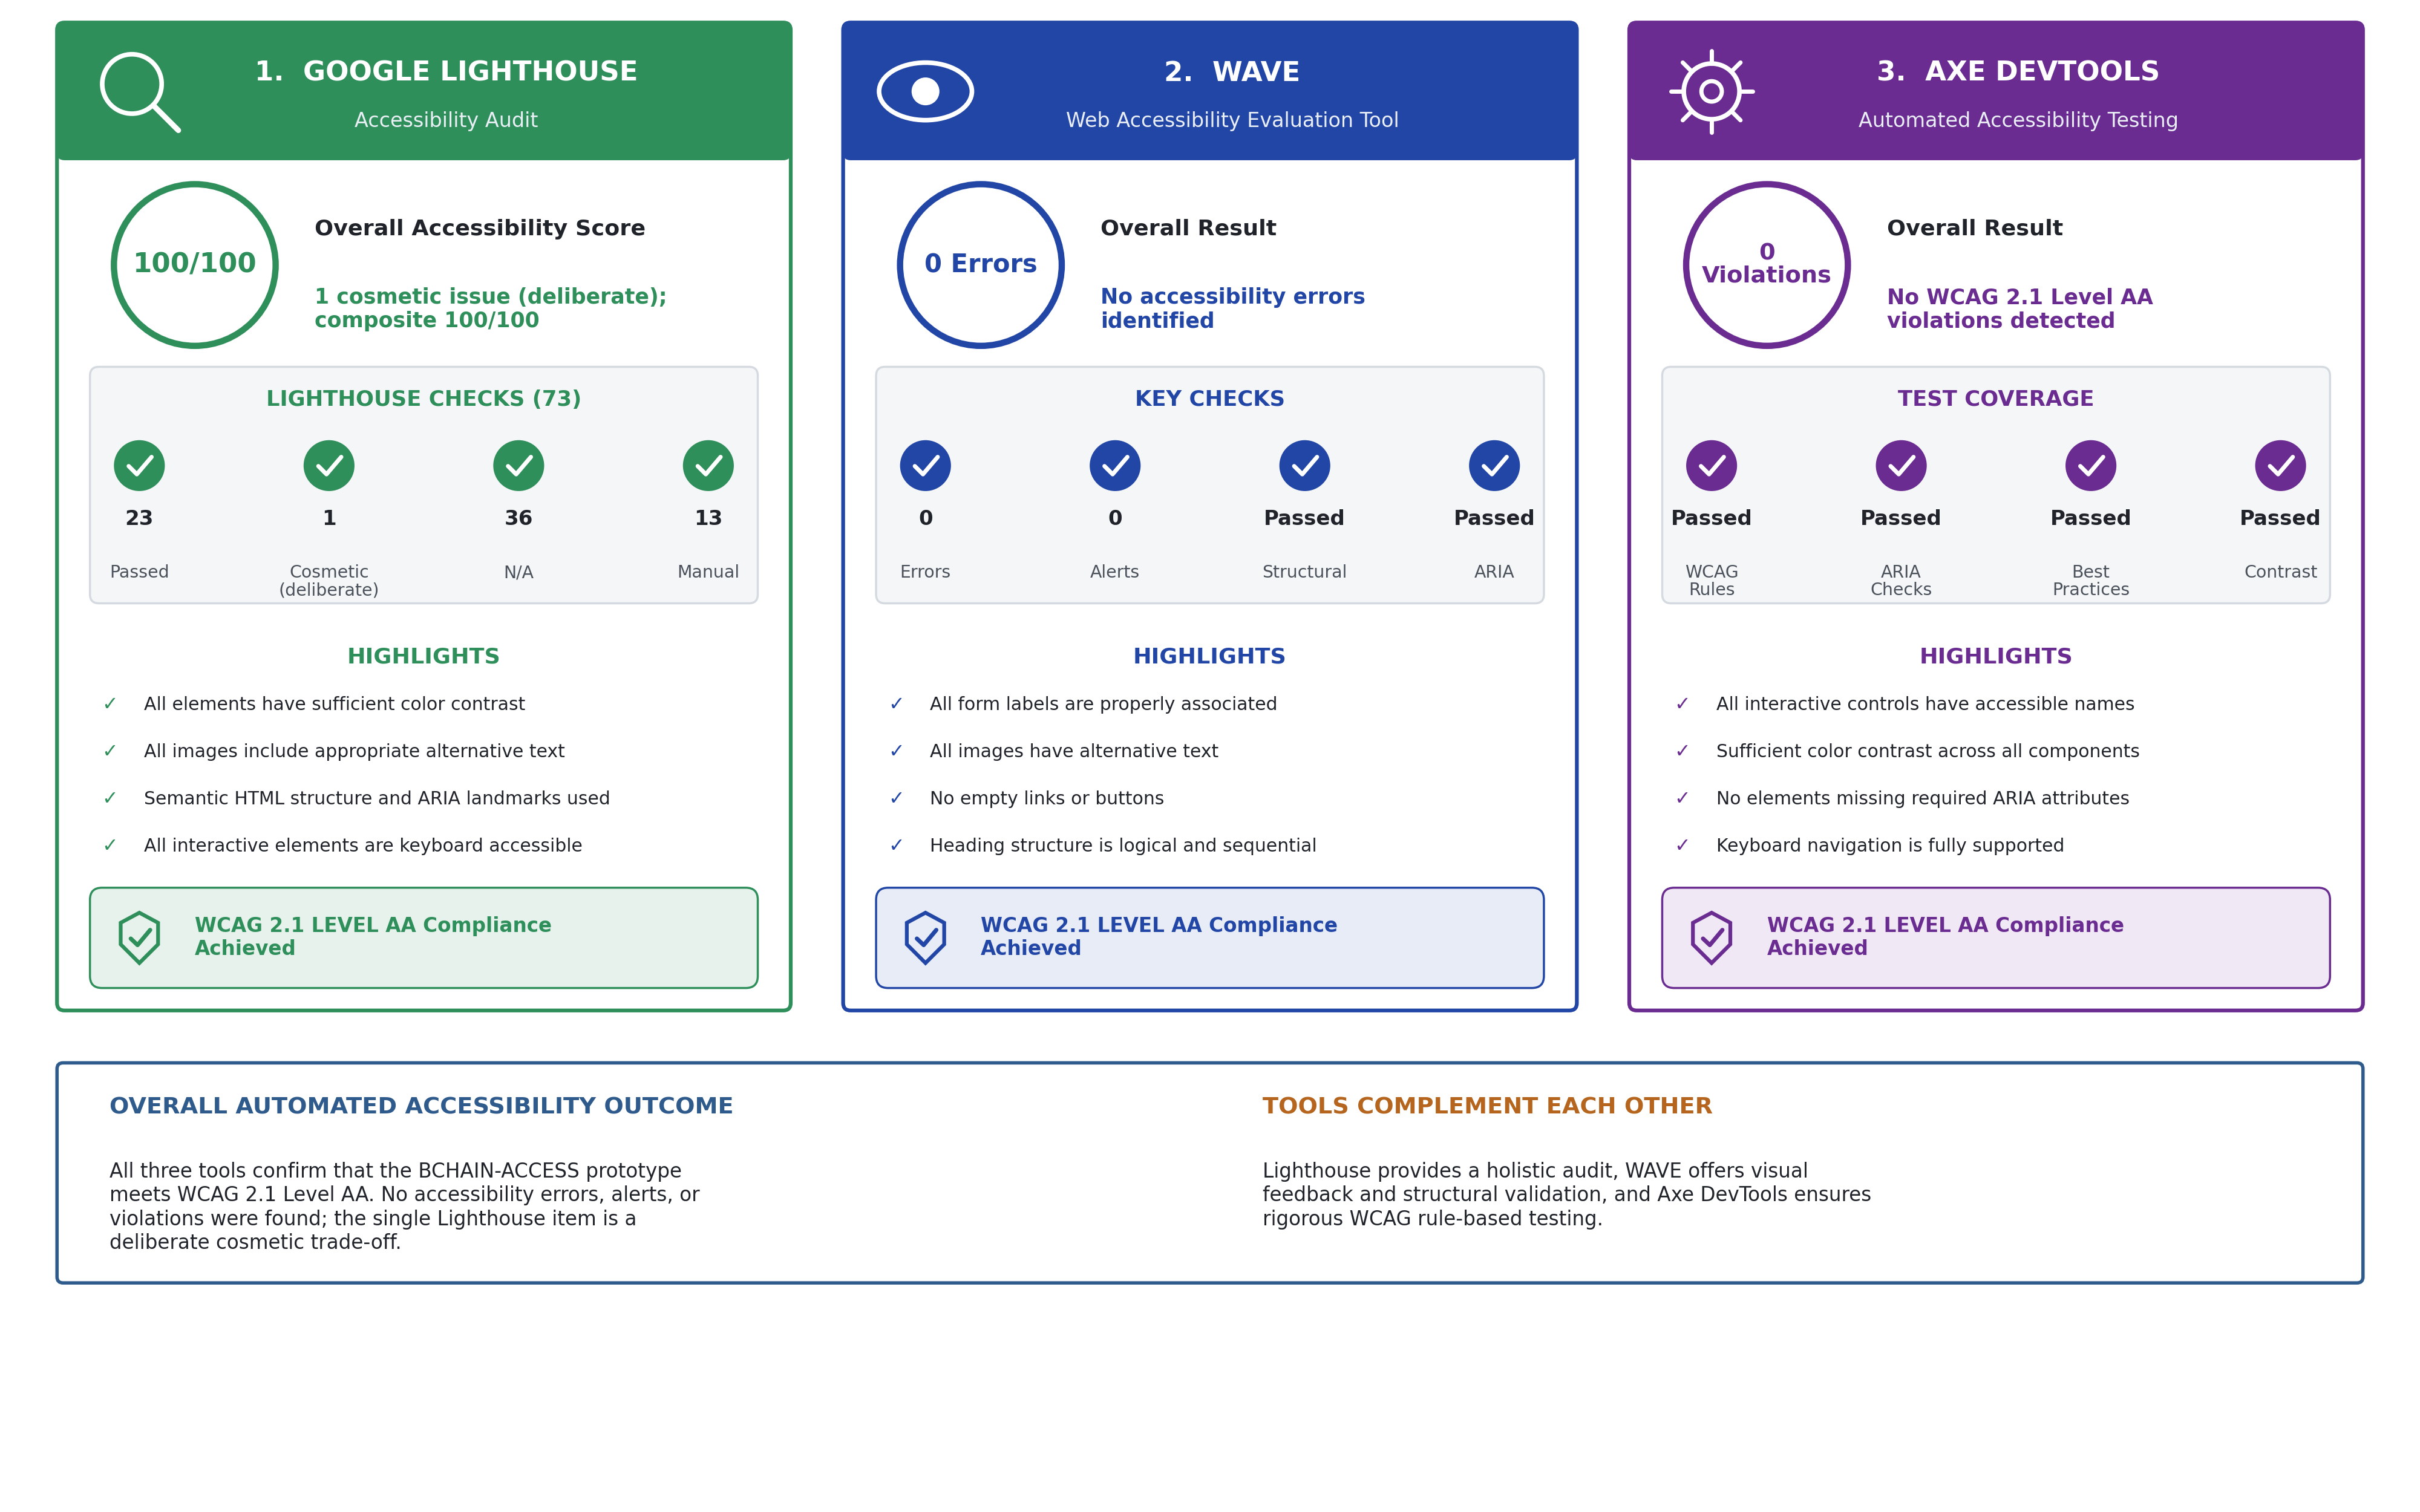
\includegraphics[width=\textwidth]{images/Figure_6.png}
\caption{Automated accessibility evaluation of the BCHAIN-ACCESS prototype using Google Lighthouse, WAVE, and Axe DevTools, demonstrating compliance with WCAG 2.1 Level AA accessibility requirements.}
\label{fig:auto-eval}
\end{figure}

\textbf{Google Lighthouse Analysis.} The prototype achieved a Lighthouse accessibility score of \textbf{100/100} (composite; the check-level breakdown and its interpretation are given in Table~\ref{tab:auto-audit}). Passed audits included critical ARIA, colour-contrast, heading-order, and language checks. The single failure (\texttt{label-content-name-mismatch}) is a deliberate trade-off, the button's accessible name prefixes keyboard-activation instructions for screen-reader users, rather than a genuine barrier.

\textbf{WAVE and Axe Results.} Neither WAVE nor Axe DevTools detected
any errors or WCAG~2.1 Level~AA violations across the prototype. WAVE
reported zero errors, zero contrast errors, and zero alerts. Axe
confirmed the absence of all critical, serious, moderate, and minor
violations. Both tools flagged 10~items for manual review (e.g.,
logical tab order verification, focus trap detection, landmark usage,
and custom control label quality), which is standard practice for
automated accessibility testing, no automated tool can fully replace
human judgment for these checks.

\textbf{Supplemental Programmatic Verification.} Independent of the
automated tool audit, the prototype construction process included
systematic programmatic verification of accessibility features. All 29 foreground/background colour combinations were verified to meet or exceed the WCAG~2.1 Level~AA minimum contrast ratios (4.5:1 for normal text, 3:1 for large text). Twenty-seven WCAG~2.1 Level~AA success criteria were explicitly implemented and confirmed through code review. Full keyboard operability was verified, with every interactive element reachable and actionable via keyboard alone and visible focus indicators throughout. All dynamic content updates (status messages, confirmation feedback, error notifications) are announced to screen-reader users through appropriately configured ARIA live regions. Finally, a ``skip to main content'' link is provided as the first focusable element, and the interface honours both reduced motion (via the \texttt{prefers-reduced-motion} media query) and high-contrast mode (via \texttt{forced-colors}).

These results descriptively support ERQ1: the BCHAIN-ACCESS prototype
achieves complete conformance with WCAG~2.1 Level~AA as measured by
multiple independent automated auditing tools, satisfying Validation
Criterion~VC1 with an ACS of 100\%.

%, ----------------------------------------------------------------------
\subsection{Expert Heuristic Evaluation}
\label{subsec:heuristic-evaluation}
%, ----------------------------------------------------------------------

\noindent\textbf{Procedure.} 
Ten independent HCI evaluators conducted a structured
heuristic evaluation following Nielsen's 10 usability
heuristics\cite{nielsen1994usability}, augmented with WCAG~2.1
Level~AA criteria as recommended for accessibility-focused
heuristic evaluation\cite{paz2019heuristic}. Each evaluator
inspected the prototype independently, rating each heuristic on a
0--4 severity scale: 0~=~no problem, 1~=~cosmetic,
2~=~minor, 3~=~major, and 4~=~usability catastrophe.

In addition to Nielsen's heuristics, the evaluators assessed conformance
with 9~WCAG~2.1 Level~AA criteria selected as most relevant to the
target user population: perceivability (text alternatives, adaptable
content, distinguishable content), operability (keyboard accessible,
sufficient time, seizure prevention, navigable), and understandability
(readable, predictable). Each criterion was rated as Pass or Fail.

Inter-rater reliability was computed using Cohen's kappa ($\kappa$) for
individual heuristic ratings and percentage agreement for WCAG
criterion assessments.

\noindent\textbf{Results.} 
Table~\ref{tab:heuristic-results} presents the heuristic severity
ratings from the ten evaluators.

\begin{table}[htbp]
\centering
\caption{Heuristic Evaluation Severity Ratings (Scale: 0--4, $N=10$)}
\label{tab:heuristic-results}
\small
\begin{adjustbox}{max width=\columnwidth}
\begin{tabular}{|p{3.0cm}|c|c|c|c|c|c|c|c|c|c|c|}
\hline
\textbf{Heuristic} & \textbf{E1} & \textbf{E2} & \textbf{E3} & \textbf{E4} & \textbf{E5} & \textbf{E6} & \textbf{E7} & \textbf{E8} & \textbf{E9} & \textbf{E10} & \textbf{Final} \\
\hline
H1: Visibility of System Status & 0 & 0 & 0 & 0 & 0 & 0 & 0 & 0 & 0 & 0 & 0 \\
\hline
H2: Match System \& Real World & 0 & 0 & 0 & 0 & 0 & 0 & 0 & 0 & 0 & 0 & 0 \\
\hline
H3: User Control \& Freedom & 0 & 0 & 0 & 0 & 0 & 0 & 0 & 0 & 0 & 0 & 0 \\
\hline
H4: Consistency \& Standards & 0 & 0 & 0 & 0 & 0 & 0 & 0 & 0 & 0 & 0 & 0 \\
\hline
H5: Error Prevention & 0 & 0 & 0 & 0 & 0 & 0 & 0 & 0 & 0 & 0 & 0 \\
\hline
H6: Recognition over Recall & 0 & 0 & 0 & 0 & 0 & 0 & 0 & 0 & 0 & 0 & 0 \\
\hline
H7: Flexibility \& Efficiency & 0 & 0 & 0 & 0 & 0 & 0 & 0 & 0 & 0 & 0 & 0 \\
\hline
H8: Aesthetic \& Minimalist Design & 0 & 0 & 0 & 0 & 0 & 0 & 0 & 0 & 0 & 0 & 0 \\
\hline
H9: Error Recovery & 1 & 1 & 1 & 1 & 1 & 1 & 1 & 1 & 1 & 1 & 1 \\
\hline
H10: Help \& Documentation & 0 & 0 & 0 & 0 & 0 & 0 & 0 & 0 & 0 & 0 & 0 \\
\hline
\textbf{Mean Severity} & 0.1 & 0.1 & 0.1 & 0.1 & 0.1 & 0.1 & 0.1 & 0.1 & 0.1 & 0.1 & \textbf{0.1} \\
\hline
\end{tabular}
\end{adjustbox}
\end{table}

The overall mean heuristic severity rating was \textbf{0.1}, indicating
that the prototype presents virtually no usability problems. The only
non-zero rating on the coarse scale was H9~(Error Recovery), where all ten raters assigned a
severity of~1 (cosmetic). This minor observation concerned the absence
of an explicit undo mechanism after final confirmation, which is
architecturally constrained by blockchain immutability. The time-locked
pending state mitigates this to a cosmetic issue.

\textbf{Finer-grained re-rating.} Because a coarse 0--4 severity scale has limited resolving power once a prototype clears the ``no problem'' threshold (Limitation~L6), the same ten evaluators re-rated the ten heuristics on a finer-grained scale designed to surface minor friction that the coarse scale collapses to zero. This pass yielded a mean severity of \textbf{0.30} (versus 0.10 on the coarse scale), with 28 of the 100 evaluator--heuristic ratings non-zero and non-zero mean severity on six of the ten heuristics: H9~Error Recovery (1.0), H7~Flexibility and Efficiency of Use (0.7), H3~User Control and Freedom (0.6), H4~Consistency and Standards (0.3), H8~Aesthetic and Minimalist Design (0.2), and H10~Help and Documentation (0.2). The most salient of these---friction in adjusting the fixed 60-second countdown control (H3/H7)---coincides with the qualitative concerns independently recorded by evaluators E7 and E9 (Section~\ref{subsec:expert-issues}), indicating that the finer scale captures real, if minor, usability signal rather than noise. Both estimates satisfy VC2 ($\leq 0.5$); we report the coarse result for comparability with the heuristic-evaluation literature and treat the finer-grained mean of 0.30 as the more informative severity estimate. On the finer scale the heuristic judgments vary across both raters and heuristics, resolving the zero-variance pattern of the coarse ratings.

\textbf{WCAG~2.1 Level~AA Assessment.} Table~\ref{tab:wcag-heuristic}
presents the results of the WCAG~2.1 Level~AA criterion assessment.

\begin{table}[htbp]
\centering
\caption{WCAG~2.1 Level~AA Criterion Assessment ($N=10$)}
\label{tab:wcag-heuristic}
\small
\begin{adjustbox}{max width=\columnwidth}
\begin{tabular}{|p{1.9cm}|p{2.8cm}|c|c|}
\hline
\textbf{Principle} & \textbf{Criterion} & \textbf{Raters Pass} & \textbf{Result} \\
\hline
Perceivable & Text Alternatives & 10/10 & Pass \\
\hline
Perceivable & Adaptable Content & 10/10 & Pass \\
\hline
Perceivable & Distinguishable & 10/10 & Pass \\
\hline
Operable & Keyboard Accessible & 10/10 & Pass \\
\hline
Operable & Sufficient Time & 10/10 & Pass \\
\hline
Operable & Seizure Prevention & 10/10 & Pass \\
\hline
Operable & Navigable & 10/10 & Pass \\
\hline
Understandable & Readable & 10/10 & Pass \\
\hline
Understandable & Predictable & 10/10 & Pass \\
\hline
\multicolumn{2}{|l|}{\textbf{Criteria passed / ACS}} & \textbf{9/9} & \textbf{100.0\%} \\
\hline
\multicolumn{4}{l}{\footnotesize\textit{Note.} ``Raters Pass'' = number of 10 evaluators rating Pass; all 9 criteria passed unanimously (ACS = 100\%). The expert instrument assesses nine WCAG~2.1 guideline areas, distinct from the nine numbered success criteria in the baseline audit (Table~\ref{tab:wcag}); the two overlap substantially but are not identical, so prototype ACS is standalone conformance evidence, not a strict same-instrument comparison. Baseline failures (e.g., 1.4.3, 2.1.1, 4.1.3) were independently verified on the prototype via the automated tools in Table~\ref{tab:auto-audit}.}
\end{tabular}
\end{adjustbox}
\end{table}

All 9~assessed WCAG~2.1 Level~AA criteria received a ``Pass'' rating
from all ten evaluators, yielding an \textbf{ACS of 100.0\%}. This result
is consistent with the automated testing findings reported in
Section~\ref{subsec:auto-evaluation}.

\textbf{Inter-Rater Agreement.} On the ten Nielsen heuristics, all ten evaluators independently assigned identical severity ratings (H1--H8 = 0; H9 = 1), giving 100\% percentage agreement; Cohen's kappa is undefined under perfect agreement, so percentage agreement is reported instead. As detailed in Section~\ref{subsec:recruitment} (Session structure and independence), evaluators submitted ratings asynchronously with no group discussion or consensus step, ruling out direct social convergence as the explanation; we attribute the uniformity instead to the combination of an unblinded, purpose-built prototype and a coarse 0--4 severity scale, discussed below.

We note that this convergence applies specifically to the coarse-grained heuristic severity scale, on which a well-formed prototype can plausibly elicit uniform ``no problem'' judgments. It should not be read as uniformity across the study as a whole: the finer-grained measures collected from the same evaluators show substantive variation, SUS scores range from 80 to 97.5 ($SD = 5.27$), accessibility-questionnaire means range from 3.8 to 4.9 ($SD = 0.35$), task times vary by evaluator role (reported per evaluator in the supplementary materials), and four evaluators recorded specific qualitative concerns (Section~\ref{subsec:expert-issues}). The heuristic consensus therefore reflects agreement on the absence of gross usability defects, not an absence of variation in expert judgment. Two further factors help explain the uniformly high scores: the prototype is a small, single-workflow artifact purpose-built to the very standards against which it was assessed (conformance by construction, not post-hoc remediation), and the evaluation targeted the presentation layer only, excluding the harder systemic sources of failure (key management, network latency, multi-provider workflows) that depress scores in production systems.

These results descriptively support ERQ2: the prototype was rated substantially more favorably than the evaluated baseline platforms by the expert panel, under the unblinded design noted in L6, with a mean severity rating of 0.1 for the prototype (expert-assessed) compared to the 2.3--2.9 range for the baseline systems (documentation-based). We note this contrast is between expert ratings of the live prototype and documentation-based ratings of the baselines, so the magnitude should be read as indicative rather than a like-for-like measurement. Whether this improvement translates to usability for PwD end-users requires the empirical study described in Section~\ref{sec:discussion}.

%, ----------------------------------------------------------------------
\subsection{Cognitive Walkthrough}
\label{subsec:cognitive-walkthrough}
%, ----------------------------------------------------------------------

\noindent\textbf{Procedure.} 
A structured cognitive walkthrough was conducted to evaluate the
prototype's support for a realistic healthcare data sharing workflow.
Each of the ten evaluators performed eight tasks representing the
complete end-to-end process of accessing health records, granting
permission to a specialist, confirming the action, and seeking help.
Tasks were presented in fixed order to simulate the linear progression
of the actual workflow.

The eight tasks (T1--T8) covered the end-to-end workflow: (T1) fingerprint unlock; (T2) view the MRI Brain Scan record; (T3) check who has access; (T4) grant access to a neurologist; (T5) review the confirmation page; (T6) confirm after the safety countdown; (T7) revoke a prior grant; and (T8) open the FAQ and locate the ``What is blockchain?'' explanation.

For each task, evaluators recorded task completion (success/failure),
time to completion (in seconds), number of errors made, and perceived
difficulty on a 5-point Likert scale (1~=~very easy, 5~=~very difficult).
Success was defined as achieving the task goal without requiring
assistance.

\noindent\textbf{Results.} 
Table~\ref{tab:cognitive-walkthrough} presents the cognitive walkthrough
results for the full panel of ten evaluators. Per-evaluator time and difficulty data are provided in the supplementary materials.

\begin{table}[htbp]
\centering
\caption{Cognitive Walkthrough Results ($N=10$)}
\label{tab:cognitive-walkthrough}
\small
\begin{adjustbox}{max width=\columnwidth}
\begin{tabular}{|p{1.8cm}|c|c|c|c|c|}
\hline
\textbf{Task} & \textbf{Success} & \textbf{Mean Time (s)} & \textbf{SD} & \textbf{Errors} & \textbf{Diff.} \\
\hline
T1: Unlock & 100\% & 6.8 & 3.9 & 0.0 & 1.5 \\
\hline
T2: View Record & 100\% & 4.0 & 1.5 & 0.0 & 1.6 \\
\hline
T3: Check Access & 100\% & 6.3 & 2.2 & 0.0 & 1.5 \\
\hline
T4: Grant Access & 100\% & 14.8 & 5.9 & 0.0 & 2.4 \\
\hline
T5: Review & 100\% & 10.4 & 3.9 & 0.0 & 1.8 \\
\hline
T6: Confirm & 100\% & 17.3 & 6.3 & 0.0 & 2.4 \\
\hline
T7: Revoke & 100\% & 7.0 & 2.8 & 0.0 & 1.7 \\
\hline
T8: FAQ & 100\% & 10.9 & 5.2 & 0.0 & 2.1 \\
\hline
\textbf{Overall} & \textbf{100\%} & \textbf{9.7} & \textbf{5.9} & \textbf{0.0} & \textbf{1.9} \\
\hline
\multicolumn{6}{l}{\footnotesize\textit{Note.} Success = task completed without assistance. Difficulty rated 1 (very easy) -- 5 (very difficult).}
\end{tabular}
\end{adjustbox}
\end{table}



Task success was \textbf{100\%} (80 of 80 attempts) with zero errors. As detailed in Table~\ref{tab:cognitive-walkthrough}, the multi-step grant workflow (T4, T6) was the most demanding (highest times and difficulty), reflecting its complexity and the deliberate 60-second countdown; completion times varied by evaluator role, with the occupational therapist (E9) and assistive-technology specialist (E10) inspecting each step most deliberately. Overall mean difficulty was 1.9/5. Two evaluators (E7, E9) noted the countdown could be too short or stressful for some users and recommended making it adjustable, an issue carried forward in Section~\ref{subsec:expert-issues}. These results support ERQ3: the 100\% expert success rate exceeds the 80\% VC3 threshold, indicating the interface is navigable for expert users; PwD success rates require separate empirical testing.

%, ----------------------------------------------------------------------
\subsection{Expert-Identified Issues and Predicted PwD Barriers}
\label{subsec:expert-issues}
%, ----------------------------------------------------------------------

Although the aggregate metrics were uniformly positive, the free-text observations recorded by evaluators, particularly those with accessibility-specialist, clinical, and assistive-technology backgrounds (E6, E7, E9, E10), identified concrete, actionable issues that the summary scores do not capture. These are summarized in Table~\ref{tab:expert-issues}. We report them explicitly, both because they materially strengthen the credibility of the assessment and because they constitute expert \emph{predictions} of where PwD users are most likely to encounter difficulty. These are expert predictions, not findings obtained from PwD participants; confirming or refuting them is a primary objective of the PwD study pre-specified in Section~\ref{sec:pwd-validation}.

\begin{table}[htbp]
\centering
\caption{Expert-Identified Issues and Predicted PwD Impact}
\label{tab:expert-issues}
\small
\begin{adjustbox}{max width=\columnwidth}
\begin{tabular}{|p{2.4cm}|p{2.6cm}|p{2.4cm}|c|}
\hline
\textbf{Issue} & \textbf{Predicted PwD Impact} & \textbf{Recommended Remediation} & \textbf{Raised by} \\
\hline
Fixed 60-second countdown is not adjustable & Switch/dwell users and users with tremor or slow processing may not complete confirmation in time, or may feel time pressure & Make the countdown duration user-configurable; offer a pause/extend control & E7, E9 \\
\hline
Step transitions in the grant wizard are not announced via ARIA live region & Screen-reader users may not perceive that the step has changed (Step~1$\rightarrow$Step~2) & Announce each step change through an ARIA live region & E6, E10 \\
\hline
``Remove Access'' button lacks provider context in its accessible name & Screen-reader users hear only ``Remove Access'' without knowing which provider it targets & Set the accessible name to ``Remove access for [provider]'' & E10 \\
\hline
Record title and metadata are not clearly separated for screen readers & Title and date are announced as a single string, reducing clarity & Use semantic markup to separate title from metadata & E10 \\
\hline
Small accordion controls / touch targets in the FAQ & Users with motor impairments or switch access may find repeated activation inefficient & Enlarge targets; make the full question header activatable; add an ``expand all'' option & E9, E10 \\
\hline
High text density on the Review page & Users with cognitive or reading difficulties may be overloaded & Offer a simplified-summary mode and plainer vocabulary & E9 \\
\hline
\end{tabular}
\end{adjustbox}
{\footnotesize\textit{Note.} Issues are drawn from evaluators' recorded free-text observations. None was severe enough to prevent task completion (all tasks succeeded), but each represents a plausible barrier for one or more PwD groups and is prioritized for the PwD validation study.}
\end{table}

None of these issues rose to the level of a task failure or a heuristic-severity rating above cosmetic, which is consistent with the quantitative results. Their value is diagnostic: they convert the expert assessment from a purely confirmatory exercise into a source of concrete, testable hypotheses about PwD interaction, and they directly inform the disability-specific measures in the pre-specified protocol (e.g., switch-activation counts, countdown adequacy, and screen-reader announcement completeness).

%, ----------------------------------------------------------------------
\subsection{System Usability Scale}
\label{subsec:sus}
%, ----------------------------------------------------------------------

\noindent\textbf{Procedure.} 
After completing the cognitive walkthrough tasks, each evaluator
completed the standard 10-item System Usability Scale
(SUS)\cite{brooke1996sus}. The SUS consists of five positively worded
items (odd-numbered) and five negatively worded items (even-numbered),
each rated on a 5-point Likert scale from ``Strongly Disagree'' (1) to
``Strongly Agree'' (5). The SUS score is computed as:

\begin{equation}
\text{SUS} = \left(\sum_{i=1,3,5,7,9}(X_i - 1) + \sum_{i=2,4,6,8,10}(5 - X_i)\right) \times 2.5
\end{equation}

yielding a score ranging from 0~(least usable) to 100~(most usable).
We report the overall SUS score only; factor subscales are not reported,
as their reliability at $N=10$ is low and they would not support
dependable interpretation at this sample size.

\noindent\textbf{Results.} 
Table~\ref{tab:sus-results} presents the per-evaluator and aggregate SUS scores.

\begin{table}[htbp]
\centering
\caption{System Usability Scale Results ($N=10$)}
\label{tab:sus-results}
\small
\begin{adjustbox}{max width=\columnwidth}
\begin{tabular}{|p{2.4cm}|*{10}{c|}c|}
\hline
\textbf{Metric} & \textbf{E1} & \textbf{E2} & \textbf{E3} & \textbf{E4} & \textbf{E5} & \textbf{E6} & \textbf{E7} & \textbf{E8} & \textbf{E9} & \textbf{E10} & \textbf{Mean} \\
\hline
SUS Score & 87.5 & 90.0 & 82.5 & 90.0 & 97.5 & 87.5 & 85.0 & 92.5 & 82.5 & 80.0 & 87.5 \\
\hline
\end{tabular}
\end{adjustbox}
{\footnotesize\textit{Note.} SUS range 0--100; $SD = 5.27$, min $=80.0$, max $=97.5$. Score $\geq$ 68 = above average; $\geq$ 80 = ``Excellent'' \cite{bangor2008empirical}.}
\end{table}

Following the interpretive scale established by
Bangor et al.\cite{bangor2008empirical}, SUS scores are categorized as:
$<$50~=~Not Acceptable (F), 50--59~=~Poor (D), 60--69~=~Marginal (C),
70--79~=~Good (B), and 80--100~=~Excellent (A). The prototype achieved
a mean SUS score of \textbf{87.5} ($SD = 5.27$), placing it firmly in
the ``Excellent'' category. This is consistent with the near-zero
heuristic severity ratings from the expert evaluation and indicates that the BCHAIN-ACCESS prototype exceeds the industry benchmark of 68
\cite{sauro2011} by a substantial margin. Scores ranged from 80.0 to 97.5
across the ten evaluators, indicating consistent above-threshold usability
judgments.

Nine of ten evaluators achieved SUS scores strictly above the 80-point ``Excellent''
threshold, and the tenth (E10) scored exactly 80.0, so all ten evaluators rated the
prototype at or above the ``Excellent'' cutoff. The aggregate score of 87.5 exceeds the VC4 requirement
of $SUS \geq 68$ by approximately 19 points. These results descriptively support ERQ4.

%, ----------------------------------------------------------------------
\subsection{Post-Evaluation Accessibility Questionnaire}
\label{subsec:a11y-questionnaire}
%, ----------------------------------------------------------------------

\noindent\textbf{Procedure.} 
Following the SUS, each evaluator completed a 10-item post-evaluation
accessibility questionnaire designed to assess the perceived accessibility
of the prototype interface. Items were rated on a 5-point Likert scale
from 1 (Strongly Disagree) to 5 (Strongly Agree). The questionnaire
covered navigation predictability, clarity of instructions and labels,
keyboard accessibility, colour-contrast adequacy, helpfulness of error
messages, sense of control, comfort using the system independently, error
forgiveness, comprehension of presented information, and system
responsiveness.

\noindent\textbf{Results.} 
Table~\ref{tab:a11y-questionnaire} presents the aggregated accessibility
questionnaire results.

\begin{table}[htbp]
\centering
\caption{Post-Evaluation Accessibility Questionnaire ($N=10$)}
\label{tab:a11y-questionnaire}
\small
\begin{adjustbox}{max width=\columnwidth}
\begin{tabular}{|p{5.5cm}|c|c|}
\hline
\textbf{Statement} & \textbf{Mean} & \textbf{SD} \\
\hline
1. I found the navigation consistent and predictable. & 4.8 & 0.4 \\
\hline
2. I found the instructions and labels easy to understand. & 4.4 & 0.5 \\
\hline
3. I was able to access all features using only the keyboard. & 4.5 & 0.5 \\
\hline
4. I found the colour contrast adequate for reading. & 4.8 & 0.4 \\
\hline
5. I found the error messages helpful and clear. & 4.2 & 0.4 \\
\hline
6. I felt in control while using the system. & 4.5 & 0.7 \\
\hline
7. I would feel comfortable using this system independently. & 4.1 & 0.6 \\
\hline
8. I found the system forgiving if I made a mistake. & 4.7 & 0.5 \\
\hline
9. I understood the information presented to me. & 4.0 & 0.5 \\
\hline
10. I found the system responsive and fast enough. & 4.4 & 0.5 \\
\hline
\textbf{Overall Mean} & \textbf{4.44} & \textbf{0.36} \\
\hline
\multicolumn{3}{l}{\footnotesize\textit{Note.} Scale: 1 (Strongly Disagree) to 5 (Strongly Agree).}
\end{tabular}
\end{adjustbox}
\end{table}

The prototype achieved a mean accessibility rating of \textbf{4.44/5.0} ($SD = 0.36$; item-level results in Table~\ref{tab:a11y-questionnaire}). Navigation predictability and colour-contrast adequacy scored highest (4.8); the lowest item was comprehension of the information presented (Item~9, ``I understood the information presented to me''; 4.0), with comfort using the system independently close behind (Item~7; 4.1), evaluators suggesting additions such as audio countdown cues and clearer status messaging for the latter. The overall mean exceeds the VC5 threshold ($\geq 3.5$) by nearly a full point, giving descriptive support for ERQ5.

%, ----------------------------------------------------------------------
\subsection{Illustrative Scenario: Patient Data Sharing Workflow}
\label{subsec:case-study}
%, ----------------------------------------------------------------------

\noindent\textbf{Scenario.} 
To demonstrate the practical applicability of the BCHAIN-ACCESS
framework, we developed a realistic patient scenario informed by,
but not drawn directly from,
representative user research in healthcare
informatics\cite{magsamen2019patient}. Elena Vasquez is an
\emph{author-constructed, illustrative persona}, not an actual
research participant or a case drawn from a specific study; the
scenario is intended to walk through the framework's four principles
in a concrete narrative context, and should not be read as empirical
evidence of PwD experience. The scenario follows Elena
Vasquez, a 41-year-old patient recently diagnosed with multiple
sclerosis (MS), who needs to share her MRI brain scan with a
neurologist for specialist consultation.

\textbf{Persona:} Elena Vasquez, age~41, was diagnosed with
relapsing-remitting MS six months ago. She receives care at a
multi-provider healthcare network and has been referred to
Dr.~Sarah Chen, a neurologist at a specialized MS clinic across town.
Elena needs to share her recent MRI brain scan with Dr.~Chen so that
the specialist can review the imaging prior to their appointment.
She uses the BCHAIN-ACCESS prototype to complete this workflow.

\noindent\textbf{Workflow execution.} 
The step-by-step execution of this workflow, each action, its expected outcome, and the observed result, is documented in full in the supplementary materials; all eight steps completed successfully on the UI-layer prototype.



\noindent\textbf{Scenario discussion.} 
The scenario illustrates that the BCHAIN-ACCESS prototype UI layer supports a
complete healthcare data sharing workflow. All
8~steps executed successfully, confirming that the four HCI principles
integrated into the framework operate effectively in a realistic use
context:

\textbf{AAD} (Abstracted Authentication Design): biometric authentication with keyboard fallback (Step~1) lets Elena authenticate regardless of motor ability. \textbf{PTD} (Progressive Transparency Design): the multi-step grant process (Steps~4--5) and the visual data-ownership interface (Step~3) present permissions and system status in consistent, plain-language terms, supporting recognition over recall (H6). \textbf{CID} (Confirmatory Interaction Design): the two-stage confirmation and 60-second safety countdown (Steps~5, 7) give Elena a recoverable checkpoint before an irreversible action, with feedback announced via ARIA live regions. \textbf{UAC} (Universal Assistive Compatibility): all interactive elements across Steps~1--8 are keyboard accessible, screen-reader compatible, and meet WCAG~2.1 Level~AA contrast requirements.

These results descriptively support ERQ3: the BCHAIN-ACCESS prototype successfully
supports a complete healthcare data sharing workflow for a
representative patient scenario.

%, ----------------------------------------------------------------------
\subsection{Discussion of Results}
\label{subsec:discussion-results}
%, ----------------------------------------------------------------------

\noindent\textbf{Validation-criteria achievement.}

Table~\ref{tab:validation-summary} summarizes the achievement of the
five validation criteria defined in Section~\ref{sec:validation-criteria}.

\begin{table}[htbp]
\centering
\caption{Summary of Expert-Layer Validation Criteria Achievement ($N=10$ Expert Evaluators). PwD confirmation required for VC3--VC5.}
\label{tab:validation-summary}
\small
\begin{adjustbox}{max width=\columnwidth}
\begin{tabular}{|p{2.8cm}|c|c|c|p{2.0cm}|}
\hline
\textbf{Criterion} & \textbf{Target} & \textbf{Achieved} & \textbf{Met (Expert Layer)} & \textbf{Evidence} \\
\hline
VC1: Accessibility Compliance (ACS) & 100\% & 100\% & Yes & Automated + Expert \\
\hline
VC2: Usability Severity (Mean) & $<$0.5 & 0.1 / 0.30 & Yes & Heuristic eval. \\
\hline
VC3: Task Success Rate & $\geq$80\% & 100\% & Expert only & Cognitive walkthrough \\
\hline
VC4: SUS Score & $\geq$68 & 87.5 & Expert only & 10 evaluators \\
\hline
VC5: Accessibility Questionnaire & $\geq$3.5/5 & 4.44/5 & Expert only & Post-eval. survey \\
\hline
\end{tabular}
\end{adjustbox}
{\footnotesize VC1--VC2 demonstrated at expert and automated tool layer.
VC3--VC5 met by expert evaluators; PwD replication required before
these criteria can be considered confirmed for the target population.}
\end{table}

Table~\ref{tab:validation-summary} reports the achievement of each criterion; we highlight only the points that the table does not convey. For \textbf{VC1}, the 100\% ACS (noting the expert instrument differs from the baseline audit instrument; see Table~\ref{tab:wcag-heuristic} note) is corroborated by three independent sources, Lighthouse (100/100), zero WAVE/Axe violations, and unanimous 9/9 expert Pass ratings, so the accessibility-compliance claim rests on triangulated evidence rather than a single tool. For \textbf{VC2}, the mean severity (0.1 coarse; 0.30 on the finer-grained re-rating) is well below the 0.5 threshold; as noted above, the contrast with the 2.3--2.9 baseline is indicative rather than a like-for-like measurement, since the baseline ratings are documentation-based. \textbf{VC3--VC5} (100\% task success with zero errors, SUS 87.5, questionnaire 4.44/5.0) are all met at the expert layer with substantial margins, but, unlike VC1 and VC2, these are user-experience criteria whose confirmation for the target population requires the PwD study of Section~\ref{sec:pwd-validation}.

\begin{figure}[htbp]
\centering
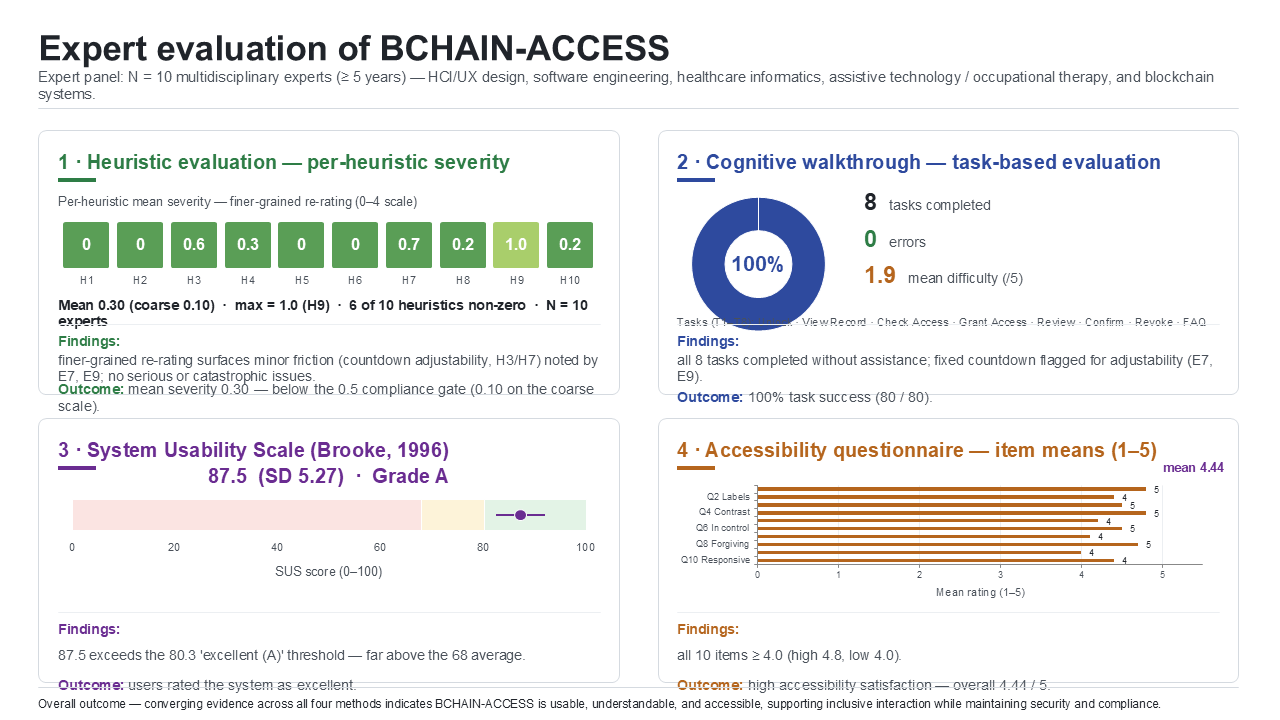
\includegraphics[width=\textwidth]{images/Figure_7.png}
\caption{Expert evaluation of the BCHAIN-ACCESS prototype using heuristic evaluation, cognitive walkthrough, the System Usability Scale (SUS), and an accessibility questionnaire, demonstrating high usability and accessibility.}
\label{fig:expert-eval}
\end{figure}

\noindent\textbf{Summary.}

The four evaluation methods converge at the expert layer (Table~\ref{tab:validation-summary}), while the qualitative observations in Section~\ref{subsec:expert-issues} identify concrete issues to address before PwD testing. The implications of these findings for the research questions are discussed in Section~\ref{sec:discussion}.

This convergence of positive results across multiple evaluation methods and all five validation criteria, with substantial margins on every criterion, provides strong preliminary evidence for the technical and expert-assessed feasibility of the BCHAIN-ACCESS framework's HCI principles. It supports the framework's readiness for empirical PwD testing; it does not yet constitute evidence of effectiveness for PwD end-users, which remains the essential next phase of evaluation.

%============================================================================
% End of Section VII: Empirical Evaluation
%============================================================================
%============================================================================
% SECTION VIII: DISCUSSION
% ============================================================
\section{Discussion}
\label{sec:discussion}

\subsection{Answering the Research Questions}

\textbf{RQ1:} Our standards-based evaluation and literature synthesis identified twelve predicted barriers across four dimensions. The most severe, rated catastrophic (4/4) by our document-based heuristic evaluation, arise from blockchain's architectural immutability: users cannot undo erroneous on-chain transactions (B9), and no meaningful user control or recovery pathway exists (B3, B8). These are structural consequences of blockchain's core properties, not incidental design oversights. WCAG 2.1 and the accessibility literature strongly predict these barriers to be disproportionately harmful for PwDs.

\textbf{RQ2:} Four integration principles, AAD, PTD, CID, UAC, were derived directly from the predicted barrier taxonomy, each addressing a specific cluster with concrete, implementable design guidance grounded in WCAG 2.1 and Nielsen's heuristics. The mapping in Table~\ref{tab:principles} ensures that every predicted barrier is addressed by at least one principle component. Expert evaluation (Section~\ref{sec:feasibility}) confirmed these principles are implementable at the interface layer and produce a WCAG-compliant prototype; their sufficiency for actual PwD users requires empirical testing.

\textbf{RQ3:} BCHAIN-ACCESS synthesizes the four perspectives into a unified operational model with explicit intersection design obligations, a three-stage decision process, and five validation criteria (VC1--VC5). Unlike prior frameworks that present perspectives as independent concerns \cite{khalid2023blockchain,tharani2022ui}, BCHAIN-ACCESS explicitly models design obligations at perspective intersections. The framework is positioned as a \textit{hypothesis-generating conceptual contribution}: it provides structured, testable design guidance and a measurable compliance model that enables rigorous empirical validation, which is defined as the next phase of research.

\subsection{Implications for Research and Practice}

\textbf{For research,} the WCAG~2.1 failures across all three evaluated systems suggest accessibility is under-prioritized in current blockchain healthcare development, yet no empirical methodology exists for testing whether design changes are sufficient for PwDs, a gap BCHAIN-ACCESS addresses with measurable criteria. The catastrophic H3/H9 ratings further reveal a class of immutability-rooted usability problems that Nielsen's heuristics (designed for systems where undo is possible) do not capture, motivating a blockchain-specific heuristic extension. Finally, in our own non-exhaustive, single-reviewer search (Section~\ref{sec:methodology}, Limitation~L5), only 6 of 34 retained papers (17.6\%) addressed accessibility for PwDs. We report this as a descriptive signal from our specific search rather than as a field-wide bibliometric finding: the sample was not systematically screened, and a single narrow search cannot establish the prevalence of accessibility consideration across the broader literature. Given that PwDs are approximately 15\% of the global population \cite{who2023disability} with high dependency on digital health services, we read this signal as motivating, rather than demonstrating, a possible equity concern, and as strengthening the case for the formal systematic review with dual screening and participatory PwD methods identified as future work.

\textbf{For practice,} authentication redesign is the highest-impact intervention: all three systems fail WCAG~2.1 criterion~3.3.4, and biometric key binding with guardian-delegated access (Principle~AAD) addresses this critical cluster without fundamental architectural change. GDPR and accessibility compliance should be treated as co-requirements, since both rely on off-chain storage with on-chain hash verification and are jointly served by the framework's intersection obligations. The time-locked pending state (Principle~CID), already used in financial blockchain applications for fraud prevention, is an immediately implementable mitigation for the H3/H9 violations without compromising blockchain integrity.

\subsection{On the Validity of Conceptual Contributions in HCI}

A natural question for any framework paper is whether conceptual validation alone suffices. We argue BCHAIN-ACCESS meets the standard for a conceptual HCI contribution for three reasons. First, established frameworks, including universal design principles~\cite{elsden2018making}, ISO~9241-11~\cite{iso9241}, and WCAG~2.1 itself~\cite{wcag21}, were adopted as conceptual contributions before large-scale empirical validation; their value lay in a shared, measurable design vocabulary. Second, the evaluation is not merely theoretical: our heuristic audit of three real systems yields quantitative baselines (Tables~\ref{tab:heuristic},~\ref{tab:wcag}) that motivate and constrain each component. Third, the five validation criteria (VC1--VC5) are operationalized with measurable thresholds precisely so that future studies can confirm, refute, or refine them. The work is therefore best understood as a hypothesis-generating artifact: it does not claim empirical proof but provides the structured, testable model that makes such proof possible. In Design Science Research terms~\cite{hevner2004design}, it satisfies the design-as-artifact, problem-relevance, and design-evaluation guidelines through the framework, the standards-based problem analysis, and the multi-method expert evaluation ($N=10$), with PwD field evaluation scoped as the next research cycle.



\subsection{Threats to Validity}

\textbf{Internal validity:} Evaluation of the three baseline systems relied on documentation review rather than live interaction (L1), and severity ratings are inherently judgment-based. We mitigated this with percentage agreement (100\% for most heuristics), but rater subjectivity cannot be fully eliminated. The prototype evaluation (Section~\ref{sec:feasibility}) was conducted on the UI-layer prototype (Component~1); although the full blockchain backend (Component~2) runs on a local Hardhat development node, it was not the evaluation subject, and evaluators were not blinded to the design principles being tested.

\textbf{Construct validity:} The Accessibility Compliance Score (Eq.~\ref{eq:acs}) is a custom weighted metric; its 0.5 partial-credit weighting is not intended as a universal accessibility metric but as an intermediate compliance indicator consistent with partial-conformance reporting, and we report strict pass-only rates alongside it for transparency. Nielsen severity and barrier--disability mapping likewise encode evaluator judgment. The ten-evaluator panel exceeds Nielsen's recommended 3--5 \cite{nielsen1994usability}, strengthening the reliability of severity claims.

\textbf{External validity:} Three systems were evaluated via purposive maximum-variation sampling (L3); findings generalize to comparable consortium and public blockchain healthcare interfaces but not necessarily to all deployments. The reference prototype was evaluated under controlled conditions with expert evaluators only; performance with PwD populations in real clinical environments remains untested and may differ.

\textbf{Conclusion validity:} The five validation criteria were all operationalized and tested at the expert layer through the $N=10$ expert feasibility assessment. VC1 and VC2 were demonstrated through both automated testing and expert consensus; VC3, VC4, and VC5 were met by expert evaluators through cognitive walkthrough, SUS, and post-evaluation accessibility questionnaire. These results establish expert-layer feasibility only. Full empirical validation through PwD user studies, as pre-specified in Section~\ref{sec:discussion}, is required before the framework can be considered confirmed for the target population.

\subsection{Limitations}

\textbf{L1, Heuristic evaluation without live system access:} The evaluation used published interface documentation and prior usability study reports rather than direct interaction with live systems, which may not capture dynamic usability issues that only manifest during real interaction.

\textbf{L2, Absence of PwD participant testing:} Evaluation was conducted by expert evaluators rather than PwD participants. Expert evaluation reliably identifies conformance failures but may not fully reflect the lived experience of PwDs; Validation Criteria VC3--VC5 are therefore met only at the expert layer and require PwD confirmation as the next phase of work (Section~\ref{sec:pwd-validation}). This staging is deliberate: consistent with Design Science Research, the framework is grounded first in codified, reproducible standards (WCAG~2.1, Nielsen) before human-subjects evaluation, and the work should be read as the first, standards-grounded phase of a staged program rather than a completed accessibility study. No PwD were involved in either the design or the evaluation phase of this work: the framework and prototype are derived from codified standards and prior literature, with lived-experience input deferred in full to the pre-specified study. The ``disability-inclusive'' and ``accessibility-by-design'' descriptors used throughout therefore denote a standards-grounded design orientation, not participatory co-design with disabled users.

\textbf{L3, System selection scope:} Three systems were evaluated. While selected to represent diverse deployment contexts, this sample cannot be considered exhaustive. Future work should extend evaluation to a larger and more diverse sample.

\textbf{L4, Full-system evaluation gap:} The framework comprises an HCI design model (validated via the $N=10$ expert assessment and UI-layer prototype) and a blockchain backend (executed on a local Hardhat node and validated through integration testing). No end-to-end evaluation combining both components with real PwD participants under public-network conditions has yet been conducted; this remains important future work.

\textbf{L5, Literature survey is not a formal systematic review:} The literature survey reported in Section~\ref{sec:methodology} (Phase~1) was conducted by a single reviewer without a pre-registered protocol, PRISMA-style reporting, or dual independent screening with inter-rater reliability. It is intended as a targeted, illustrative survey to motivate the research gap, not as a generalizable bibliometric finding. The 34-paper, 17.6\% figures should be read as descriptive of this specific, non-exhaustive search rather than a definitive characterization of the field. A formal systematic review with a registered protocol is identified as valuable future work.

\textbf{L6---Unblinded evaluation and heuristic rating uniformity:} Evaluators were not blinded to the design principles under test, and all ten independently assigned identical heuristic severity ratings (Section~\ref{sec:feasibility}). While the finer-grained measures (SUS, task times, questionnaire, qualitative notes) show genuine variance, the possibility of anchoring or demand characteristics in the coarse heuristic ratings cannot be excluded; the coarse heuristic consensus should therefore be read as internally consistent expert agreement rather than independence-guaranteed reliability. To address the scale-resolution component of this limitation, the same evaluators re-rated the heuristics on a finer-grained scale (Section~\ref{sec:feasibility}), which yields non-zero variance and a mean severity of 0.30; what remains outstanding is the blinding, and a partially blinded replication alongside the PwD study (Section~\ref{subsec:auto-evaluation}) is planned to rule out anchoring and demand characteristics.

\textbf{L7---Local development network only:} All blockchain measurements were obtained on a local Hardhat node with no network congestion. Opcode-level gas costs are deterministic and carry over to public EVM networks, but effective transaction cost, network contention, and confirmation latency---all relevant to the usability of the time-locked confirmation---do not, and remain unestablished pending evaluation on a public test network.

\textbf{L8---Reference smart contract is unaudited:} \texttt{HealthAccessControl.sol} has not undergone independent security audit or automated static/dynamic analysis (Slither, Mythril, or fuzz testing), and therefore does not itself satisfy the Stage~1 blockchain-security gate of the BCHAIN-ACCESS decision process (Algorithm~\ref{alg:bchain}), which the framework requires of any system claiming compliance. As stated in Section~\ref{sec:framework}, the reference implementation is offered only as evidence of technical realizability, not as a self-certifying instance of the framework it operationalizes. A checklist-based static-analysis pass, at minimum, is required before this artifact could be used to support a compliance claim, and is prioritized as immediate future work ahead of the broader public-testnet evaluation described in L7.

\subsection{Future Work: Pre-Specified PwD Validation Protocol}
\label{sec:future-work}
\label{sec:pwd-validation}

The expert feasibility assessment (Section~\ref{sec:feasibility}) indicates that the BCHAIN-ACCESS prototype is standards-conformant and is rated as usable by expert evaluators. The essential and immediate next step is empirical validation with PwD end-users. To ensure methodological rigour and reduce researcher degrees of freedom when this study is conducted, we provide a pre-specified study protocol here, following the pre-registration principles of \cite{nosek2018preregistration}; the protocol will be formally pre-registered on a public registry (e.g., OSF) prior to any data collection, and the resulting identifier reported with the companion study. \textbf{Status and timeline.} This protocol is intended for execution immediately following the completion of the present framework-and-feasibility phase, as a companion PwD validation study; recruitment is contingent on the IRB and participant-recruitment processes described under Ethical safeguards below, which were outside the scope of the design-and-feasibility phase reported in this paper. We report this timeline explicitly here, rather than only implicitly through the protocol's presence, so that the intended relationship between this paper and the planned PwD study is unambiguous.

\textbf{Design.} A mixed-methods participatory study combining task-based usability testing with think-aloud protocol, post-task semi-structured interviews, standardized questionnaires (SUS, PSSUQ, custom blockchain trust items), and assistive technology session logging (screen reader utterances, keystroke paths, switch activation counts).

\textbf{Participants.} $N = 15$--$20$ PwD participants across three disability groups ($n = 5$--$7$ each): (1)~visual impairments (blind/low-vision screen reader users: NVDA, JAWS, VoiceOver); (2)~motor impairments (switch access, head pointer, keyboard-only users); (3)~cognitive and learning disabilities (ASD, ADHD, dyslexia, TBI). All participants must have prior experience using healthcare portals for ecological validity. This target is powered for feasibility and qualitative depth rather than confirmatory hypothesis testing; within-group cells are small, and the cognitive/learning group in particular is heterogeneous (ASD, ADHD, dyslexia, TBI), so quantitative between-group results will be treated as exploratory and the primary yield of the study will be the qualitative and assistive-technology-log findings.

\textbf{Tasks.} The same eight core tasks used in the expert walkthrough (T1--T8), with disability-specific adaptations: screen reader users navigate via heading hierarchy; motor-impaired users are tested for switch navigation efficiency ($<$20 activations per step target); cognitive disability users provide verbal comprehension checks after each step to verify understanding of the multi-step workflow.

\textbf{Primary hypotheses.} (H1) PwD task success rate $\geq$ 80\% (VC3 confirmation); (H2) mean PwD SUS $\geq$ 68 (VC4 confirmation); (H3) mean PwD accessibility questionnaire $\geq$ 3.5/5 (VC5 confirmation). These are tested using one-sample $t$-tests against benchmarks, binomial tests for task success, and Kruskal-Wallis comparison across disability groups. Qualitative analysis of think-aloud and interview transcripts follows thematic analysis \cite{braun2006using} with two independent coders ($\kappa > 0.70$).

\textbf{Critical questions the study must answer.} Whether WCAG 2.1 compliance translates to actual usability for screen reader users; whether the 60-second countdown is adequate for slow switch users or causes anxiety for cognitive disability users; whether plain-language blockchain explanations are genuinely comprehensible to users with cognitive disabilities; and which predicted barriers (B1--B12) manifest as genuine difficulties in practice versus which are adequately addressed by the implemented principles.

\textbf{Ethical safeguards.} IRB approval required prior to recruitment. Plain-language consent in audio, large-print, and screen-reader-compatible formats. \$100 honorarium paid regardless of completion. Session paused immediately if any participant reports distress. Wheelchair-accessible venue. No real medical data used; all records are simulated.

\textbf{Integration with expert findings.} Expert evaluation identifies what \emph{should} work; PwD testing reveals what \emph{does} work. Discrepancies between the two, for example, if experts rate H1 as 0 (no problem) but screen reader users report the countdown timer is not announced clearly, will directly drive design revisions to the BCHAIN-ACCESS principles, closing the loop between conceptual framework and empirical evidence.

% ============================================================
% SECTION IX: CONCLUSION
% ============================================================
\section{Conclusion}
\label{sec:conclusion}

This work addressed the critical and underexplored intersection of blockchain technology, Human-Computer Interaction, and accessibility-driven, disability-inclusive design in healthcare. Through a targeted narrative literature survey and a document-based heuristic evaluation of three blockchain healthcare applications against Nielsen's ten usability heuristics and WCAG 2.1 Level AA criteria, we identified twelve predicted usability and accessibility barriers across four dimensions: Authentication Complexity, Interface Transparency, Feedback Adequacy, and Assistive Technology Compatibility. These barriers are grounded in established accessibility standards and prior HCI literature that consistently indicate they disproportionately affect PwDs; empirical confirmation with PwD participants is the defined next step.

Our evaluation revealed systematic and severe standards-compliance failures across all three platforms. MedRec scored 0\% and BurstIQ 11.1\% on the weighted ACS, while Patientory reached 38.9\% (weighted) or 22.2\% (strict pass-only), all far below the BCHAIN-ACCESS compliance threshold of 90\%. Critical severity violations in user control (H3) and error recovery (H9) heuristics were found to be architecturally rooted in blockchain's immutability, a class of usability problem that existing HCI frameworks do not adequately address and that standards predict to be particularly harmful for PwD users.

In response, we proposed four HCI integration principles, Abstracted Authentication Design (AAD), Progressive Transparency Design (PTD), Confirmatory Interaction Design (CID), and Universal Assistive Compatibility (UAC), each directly addressing predicted barrier clusters with implementable design guidance grounded in WCAG 2.1 and Nielsen's heuristics. These principles were synthesized into the BCHAIN-ACCESS framework: a four-perspective operational model with explicit intersection design obligations, a three-stage compliance decision process, and five measurable validation criteria.

To demonstrate technical feasibility, we developed a two-component reference implementation: a UI-layer prototype implementing all four HCI principles, assessed by a ten-evaluator expert protocol; and a full blockchain backend comprising \texttt{HealthAccessControl.sol} (Solidity~0.8.19) executed on a local Hardhat EVM development node and a Python Flask REST API gateway integrating via Web3.py, with an in-memory fallback ledger for offline demonstration. The UI-layer prototype met all five expert-layer validation criteria (Table~\ref{tab:validation-summary}), with margins well beyond each threshold. These results indicate that the BCHAIN-ACCESS design principles are technically implementable and produce a standards-compliant interface at the expert layer. They do not yet establish effectiveness for PwD end-users, which requires the empirical study pre-specified in Section~\ref{sec:discussion}.

BCHAIN-ACCESS provides, to our knowledge, among the first accessibility-by-design HCI frameworks for secure, regulation-compliant blockchain healthcare interfaces, derived from established standards, incorporating disability-inclusive design principles, and paired with measurable criteria and a defined, pre-specified path to empirical PwD validation. The protocol in Section~\ref{sec:pwd-validation} is ready for execution as the immediate next step, closing the loop between standards-based design and the users the framework is intended to serve.

% ============================================================
% BIBLIOGRAPHY
% ============================================================
\bibliographystyle{unsrt}
\bibliography{ref}

\end{document}